\documentclass[10pt,journal]{IEEEtran}

\usepackage{lineno,hyperref}
\modulolinenumbers[5]



\usepackage{graphicx} % for pdf, bitmapped graphics files
\usepackage{epsfig} % for postscript graphics files
%\usepackage{mathptmx} % assumes new font selection scheme installed
%\usepackage{times} % assumes new font selection scheme installed
\usepackage{amsmath} % assumes amsmath package installed
\usepackage{amssymb}  % assumes amsmath package installed
\usepackage{epstopdf}
\usepackage{mathtools}
\usepackage{multirow}
%\usepackage[markup=underlined]{changes}
%\usepackage[final]{changes}
\usepackage{array}
\usepackage{siunitx}
\usepackage{tikz}
\usepackage{mathrsfs}
\usepackage{tabularx}
\usepackage{amsthm}
\usepackage{url}
\usetikzlibrary{calc}
\usetikzlibrary{positioning}
\usetikzlibrary{arrows}
\usetikzlibrary{shapes}
\usetikzlibrary{fit}
\newtheorem{rem}{Remark}
\newtheorem{assm}{Assumption}
\newtheorem{alg}{Algorithm}
\newtheorem{theorem}{Theorem}
\newtheorem{lemma}{Lemma}
\newtheorem{corollary}{Corollary}
\usepackage{algpseudocode}
\usepackage{float}
\usepackage{xcolor}

\usepackage{svg}
\usepackage{psfrag}

\usepackage{pgfplots}
\usetikzlibrary{calc}
\pgfplotsset{compat=1.8}

\definecolor{line1}{cmyk}{0.02,0.16,1,0}
\definecolor{line2}{cmyk}{0.86,1,0.03,0.01}

\graphicspath{{Figures/}}

\newcommand{\ego}{\textrm{ego}}
\newcommand{\other}{\textrm{other}}
\newcommand{\nth}[1]{$#1^{\textrm{th}}$}
\newcommand{\actseq}[1]{$\boldsymbol{\gamma_{t}}[#1] = \left\{\gamma_{t}[#1],\,\gamma_{t+1}[#1],\,\cdots,\,\gamma_{t+N-1}[#1]\right\}$}
\newcommand{\actseqk}[2]{$\boldsymbol{\gamma^{\left(#2\right)}_{t}}[#1] = \left\{\gamma^{\left(#2\right)}_{t}[#1],\,\gamma^{\left(#2\right)}_{t+1}[#1],\,\cdots,\,\gamma^{\left(#2\right)}_{t+N-1}[#1]\right\}$}


%%%%%%%%%%%%%%%%%%%%%%%

%\definechangesauthor[color=Red]{RS}
%\definechangesauthor[color=Blue]{CM}

\begin{document}
	
	\title{Robust Game-Theoretic Decision-Making for Autonomous Vehicles}

	\thispagestyle{empty}
	% \pagestyle{empty}

	%% Group authors per affiliation:
	\author{
		Gokul S.~Sankar,  Kyoungseok Han and Ilya Kolmanovsky% <-this % stops a space 
		\thanks{Gokul~S.~Sankar,  Kyoungseok Han and Ilya Kolmanovsky are with the Department of Aerospace Engineering, University of Michigan, Ann Arbor, MI, USA. Emails: {\tt\small ggowrisa@umich.edu} (G.~Sankar), 
			{\tt\small kyoungsh@umich.edu} (K.~Han) and  {\tt\small ilya@umich.edu} (I.~Kolmanovsky) }%
	}

	\maketitle
	%==========================================================================%
	
	
	
	\begin{abstract}
	This paper proposes a robust decision-making strategy for autonomous vehicles based on the game theory. Autonomous vehicles should be controlled by sophisticated negotiation skills with the other road participants, e.g., human-driven vehicles, pedestrians. In this paper, by modeling the interactions between the vehicles, autonomous vehicle can make reasonable decision that is not too conservative or aggressive. The behavior of the vehicles is modeled by cognitive hierarchy theory, e.g., level-\textit{k} framework, which demonstrates its effectiveness when describing human thinking process. By inferring other vehicle's thoughts, autonomous vehicle can avoid the biased decision, i.e., conservative or aggressive. The effectiveness of the proposed approach is verified with the lane change scenario at the high-way.
	
	\end{abstract}
	
	

	%==========================================================================%
	
	\section{Introduction}
	\label{sec:intro}

	Despite many recent advances in connected and automated vehicles (CAVs) technology, the full automation systems that can provide the similar or better driving proficiency compared to the human drivers are still inherently flawed to be deployed in the market \cite{Okuda2014}. One of the most significant challenges is to plan the motion of the automated vehicles at the mixed-traffic conditions where the automated car coexists with the human-driven vehicles \cite{Lazar2018}. In particular, describing the human decision-making process is the most difficult since the humans do not always exhibit the optimized behavior due to limited rationality \cite{Griffiths2015}. In order to ensure the safety, a conservative driving policy of the automated vehicles where the all possible driving situations are considered has been suggested \cite{Claussmann2015, Brechtel2014}, but it may cause the disharmony with the human drivers. That is, too conservative behavior of the automated vehicles sometimes causes adverse effect on traffics, e.g., road congestion, car accidents, due to the uncertainties of the human drivers.
	
	If the human-driven vehicle's response according to traffics, i.e., behavior of the surrounding vehicles, can be predicted, far less conservative motion planning of the automated vehicle can be designed \cite{Sadigh2016}. As mentioned, however, modeling of the interaction between the vehicles may not very accurate. Moreover, since the communication time with the surrounding vehicles in reality is not sufficient to build the deterministic human driver models.
	
	To overcome such shortcomings, we exploit the ``level-\textit{k} game theory'' framework where the human thought processes in strategic games, i.e., driving at the mixed-traffics, are modeled in hierarchical structure \cite{Stahl1993}. The game theoretic approach has already proved its effectiveness when describing the interactions between the vehicles \cite{Li2017, Li2018, Tian2018}. Although these approaches effectively describe rational decision-making for the human-driven vehicles, the model uncertainties that affect to the vehicle position are not considered. Therefore, it is assumed that the center of gravity of the vehicle follows the deterministic kinematic model with the constant safety constraint that prevents the physical safety violation between the vehicles, and depending on the size of the safety constraint, the level of conservatism in the autonomous vehicle's motion is determined. 
	
	In this paper, we adaptively adjust the safety constraint sizes of the interactive human-driven vehicles according to the confidence level to establish a balanced motion planning between the aggressive and conservative motion planning. The interactive vehicle's aggressiveness level is estimated and it is proportional to the size of safety constraint of the human-driven vehicle. Based on this, the autonomous vehicle's future trajectory is planned, which maximizes the cumulative reward. In \cite{Jin2019}, the caution level of the human-driven vehicle is used to describe the aggressiveness of the HDV, but only constant caution level is assumed, which eventually determine the level of conservatism of AV. To resolve this, we incorporate the level-\textit{k} game theory with the caution level so that adaptive caution level is available, which enables adjustable motion planning of AV depending on the interactive vehicle's aggressiveness.
	
	The contributions of this paper are summarized as follows. Firstly, we modeled the human-driven vehicle's decision-making processes at high way using game theory, representing the a degree of the aggressiveness. Secondly, the uncertainties that is imposed in vehicle position is represented by the identified drivers aggressiveness and these bounds are utilized to make the robust decision-making strategy for the autonomous vehicles. Lastly, we verify the benefit of the proposed approach through simulations when comparing with the results that do not consider the position uncertainty.
	
	The rest of the paper is organized as follows. In Section II, the vehicle dynamic model with the bounded uncertainty is introduced. We next present the game-theoretic decision making algorithm and motion planning procedure in Section III, the effectiveness of the proposed approach is described in Section IV, and the paper is concluded in Section V.
	
	\subsection{Notation}



	%==========================================================================%

	\section{Probelm statement}
	\label{sec:problem_statement}
	
	As illustrated in Fig.~\ref{fig:lane_changing}, depending on the motions of interactive vehicles (red), the autonomous vehicle can plan the different motions. If the interactive vehicles behave aggressively, the AV should choose the conservative motion planning, and vice versa. In addition, to avoid the too conservative or aggressive driving policy, the balanced motion planning is preferred in the actual application.
	
	The problem we treat is to model the intent of the interactive vehicles using game theoretical approach, then AV exploits the estimated interactive vehicle's driving intention when making the decision in real-time. The confidence level of the estimated intention is represented by dashed-dotted boxes in Fig.~\ref{fig:lane_changing} and their sizes are adjusted adaptively according to the confidence levels.

	\begin{figure}
		\begin{centering}
			\begin{tikzpicture}
			
			\node (rect) [draw =none, very thin, fill = white, minimum width = 8.25cm, minimum height = 3cm, inner sep = 0pt] {};
			
			\node (off_road_north) [draw, very thick, fill = black, minimum width = 8.25cm, minimum height = 0.1mm, inner sep = 0pt, above  = 0mm of rect] {};
			
			\node (off_road_south) [draw, very thick, fill = black!60!green, minimum width = 8.25cm, minimum height = 0.1mm, inner sep = 0pt, below  = 0mm of rect] {};
			
			
			\draw  [loosely dashed, thick] (rect.west) -- (rect.east);
			\node (blue)	[below left = -1.25cm and -2.2cm of rect]{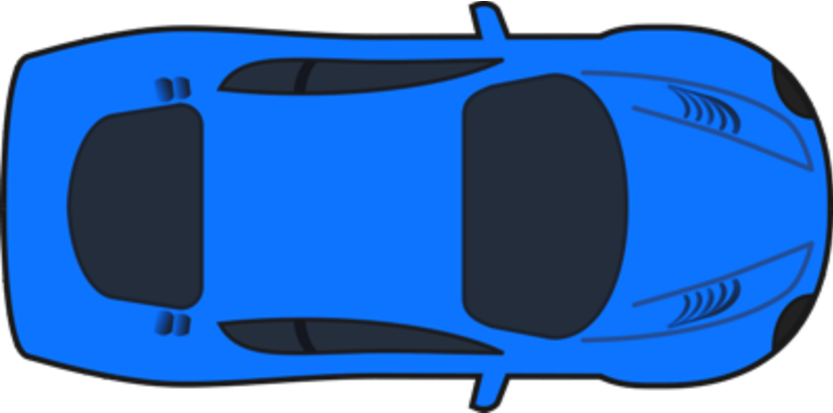
\includegraphics[scale=0.1]{blue_car.pdf}};
			\node (red1) [above left = -1.25cm and -1.8cm of rect] {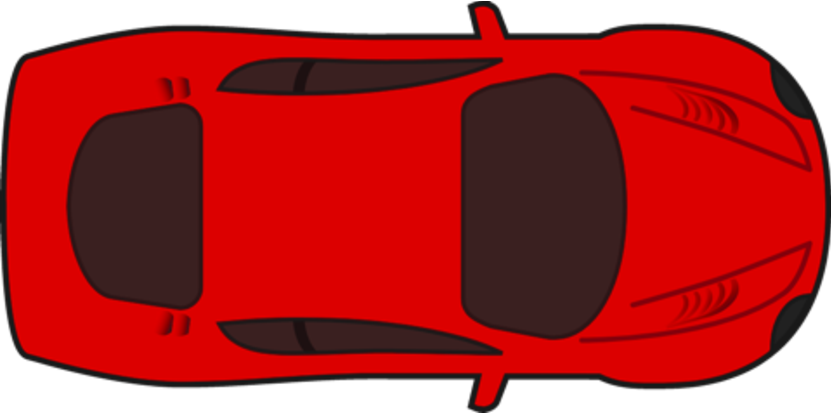
\includegraphics[scale=0.1]{red_car.pdf}};
			\node (red2)	[above right = -2.75cm and -2cm of rect]{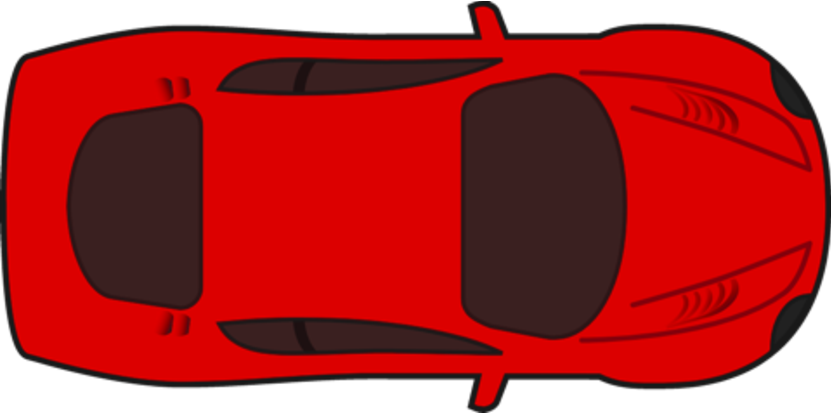
\includegraphics[scale=0.1]{red_car.pdf}};
			
			\node (mid3)	[above left = -1.58cm and -5.9cm of rect, minimum width = 0cm, minimum height = 0cm, inner sep = 0pt] {};
			\node (mid2)	[above left = -1.56cm and -4.9cm of rect, minimum width = 0.cm, minimum height = 0.cm, inner sep = 0pt] {};
			\node (mid1)	[above left = -1.56cm and -3.9cm of rect, minimum width = 0.cm, minimum height = 0.cm, inner sep = 0pt] {};
			
			
			
			
			\node (off_road_north) [draw = none, very thick, fill = black!60!green, minimum width = 8.25cm, minimum height = 1cm, inner sep = 0pt, above  = 0mm of rect, fill opacity=0.6] {};
			
			\node (off_road_south) [draw = none, very thick, fill = black!60!green, minimum width = 8.25cm, minimum height = 1cm, inner sep = 0pt, below  = 0mm of rect, fill opacity=0.6] {};
			
			
			\node (final)	[draw, circle, above right = -0.83cm and -0.5cm of rect, minimum width = 0.cm, minimum height = 0.cm, inner sep = 0pt] {};
			
			\node (final3)	[draw,  above right = -0.83cm and -1.5cm of rect, minimum width = 0.cm, minimum height = 0.cm, inner sep = 0pt] {};
			\node (final2)	[draw, circle, above right = -0.83cm and -2.5cm of rect, minimum width = 0.cm, minimum height = 0.cm, inner sep = 0pt] {};
			\node (final1)	[draw, circle, above right = -0.83cm and -3.5cm of rect, minimum width = 0.cm, minimum height = 0.cm, inner sep = 0pt] {};
			
			
			\node (breakaway1)	[draw, circle,  below left = -0.83cm and -3cm of rect, minimum width = 0.cm, minimum height = 0cm, inner sep = 0pt]{};
			\node (breakaway2)	[draw, circle,  below left = -0.83cm and -4cm of rect, minimum width = 0.cm, minimum height = 0cm, inner sep = 0pt]{};
			\node (breakaway3)	[draw, circle,  below left = -0.83cm and -5cm of rect, minimum width = 0.cm, minimum height = 0cm, inner sep = 0pt]{};		
			
			\draw [rounded corners,color=cyan,line width=3pt] (blue) .. controls (breakaway1) ..  (mid1) .. controls (final1) .. (final2) -- (final);
			\draw [rounded corners,color=line1,line width=3pt] (blue) .. controls (breakaway2) ..  (mid2) .. controls (final2) .. (final3) -- (final);
			\draw [rounded corners,color=line2,line width=3pt] (blue) .. controls (breakaway3) ..  (mid3) .. controls (final3) .. (final) ;

			\node [draw, fill = none, minimum width = 1.5cm, minimum height = 0.75cm, inner sep = 0pt, below left = -2.32cm and -1.19cm of blue, thin, dash dot, color = red] {};
		
			\node [draw, fill = none, minimum width = 1.5cm, minimum height = 0.75cm, inner sep = 0pt, below left = -0.86cm and -1.57cm of red2, thin, dash dot, color = red] {};
			
			\node [draw, fill = none, minimum width = 1.5cm, minimum height = 0.75cm, inner sep = 0pt, below left = -0.86cm and -1.57cm of blue, thin, dash dot, color = blue] {};
			
			\node[above left = -1.15cm and -2cm of blue,]{A};
			\node[above left = -1.15cm and -2.75cm of blue,]{A1};
			\node[above left = -1.15cm and -3.75cm of blue,]{A2};
			\node[above left = -1.15cm and -4.75cm of blue,]{A3};
			%		
			\node[above left = 1.15cm and -4.5cm of blue,]{B1};
			\node[above left = 1.15cm and -5.5cm of blue,]{B2};
			\node[above left = 1.15cm and -6.5cm of blue,]{B3};
			\node[above left = 1.15cm and -7.5cm of blue,]{B};
			
			\end{tikzpicture}
			\par
		\end{centering}
	\protect\caption{Possible lane changing sequences; ``aggressive motion planning"= \{(A,A1),\,(A1,B1),\,(B1,B)\}, ``balanced motion planning"=$\{\left(A,A2\right),\,\left(A2,B2\right),\,\left(B2,B\right)\}$ and ``conservative motion planning"=$\left\{\left(A,A3\right),\,\left(A3,B3\right),\,\left(B3,B\right)\right\}$ that can be chosen by the autonomous vehicle (blue) based on the motion of other non-autonomous vehicles (red).}
	\label{fig:lane_changing}
	\end{figure}
	
	
	%==========================================================================%

	\section{Vehicle dynamic model}
	\label{sec:model}

	The  vehicle dynamics are represented by the following discrete model \cite{Kong2015}

	\begin{subequations}
		\begin{align}
			x\left(t+1\right) & = 	x\left(t\right) + v\left(t\right) \cos\left(\psi \left(t\right) + \beta \left(t\right) \right) \Delta t + w_x\left(t\right)\\ 
			y\left(t+1\right) & = 	y\left(t\right) + v\left(t\right) \sin\left(\psi \left(t\right) + \beta \left(t\right) \right) \Delta t + w_y\left(t\right) \\ 
			\psi\left(t+1\right) & = 	\psi\left(t\right) + \frac{v\left(t\right)}{l_r} \sin\left( \beta \left(t\right) \right) \Delta t \\ 
			v\left(t+1\right) & = 	v\left(t\right) + a\left(t\right)  \Delta t\\
			\beta\left(t\right) & = \arctan\left(\frac{l_r}{l_r+l_f}\tan\left(\delta_f\left(t\right)\right)\right),
		\end{align}
	\label{eq:mod}
	\end{subequations}


	\noindent where  $t$ denotes the discrete time instant; the pair $\left(x\left(t\right),\,y\left(t\right)\right)$  represent the global position of the center of mass of the vehicle; the vehicle's speed is denoted by $v\left(t\right)$; 	$\beta\left(t\right)$ is the angle of $v\left(t\right)$ with respect to the longitudinal axis of the vehicle; $\psi\left(t\right)$ denotes the vehicle’s yaw angle (the angle between the vehicle’s heading direction and the global x-direction); $a\left(t\right)$ denotes the vehicle’s acceleration at time $t$;  $\Delta t$ denotes the time step size; $\delta_f\left(t\right)$  represents the front steering angle; and  $l_f$  and $l_r$  are the distance of the center of the mass of the vehicle to the front and rear axles, respectively; $w_x\left(t\right)$  and $w_x\left(t\right)$ denote the uncertainty in the position of the center of mass, respectively. It is assumed the uncertainties originate from a closed and compact disturbance set, ${\mathcal{W}} \coloneqq  \left\{ w = \left(w_x,\,w_y\right) |\zeta w\leq\theta,\,\zeta\in\mathbb{R}^{a\times 2},\,\theta\in\mathbb{R}^{b}\right\}$, with $b \in 2\mathbb{Z}^{+}$. The disturbance set is assumed to contain the origin. Furthermore, it is assumed that the rear wheels cannot be steered. Therefore, the control input to the model \eqref{eq:mod}, represented by $\gamma\left(t\right) = \left(a\left(t\right),\, \delta_f\left(t\right)\right)$, is the acceleration and front steering angle pair. 

	
	%==========================================================================%

	
	\section{Game-theoretic decision making}
	\label{sec:controller}

	At each time instant, each vehicle selects an input pair from the finite action set, $ \boldsymbol{\Gamma} = \left\{\left(0,\, 0\right),\,\left(0,\, \delta_{f,\,\textrm{nom}}\right),\,\left(0,\, -\delta_{f,\,\textrm{nom}}\right),\,\left(a_{\textrm{nom}},\, 0\right),\,\left(-a_{\textrm{nom}},\, 0\right),\right.$ $\left.\left(a_{\max},\, 0\right),\,\left(-a_{\max},\, 0\right),\,\left(a_{\textrm{nom}},\, \delta_{f,\,\max}\right),\,\left(a_{\textrm{nom}},\, -\delta_{f,\,\max}\right)\right\}$, where $a_{\textrm{nom}}$, $\delta_{f,\,\textrm{nom}}$ and $a_{\max}$, $\delta_{f,\,\max}$ are the nominal and maximum acceleration, front steer angle, respectively. The inputs pairs in $ \boldsymbol{\Gamma}$ correspond to the actions, \{``maintain", ``turn slightly left", ``turn slightly right", ``accelerate", ``decelerate", ``maximum acceleration", ``maximum deceleration", ``turn left and accelerate", `` turn right and accelerate'' \}, respectively. The input pair to be applied at every time step is decided based on optimizing a reward function.
	


	\subsection{Action choice}
	\label{sec:action_choice}
	
	The decision making process of the vehicle in choosing the optimal input pair follows a receding horizon strategy. A sequence of actions, $\boldsymbol{\gamma_{t}} = \left\{\gamma_{t},\,\gamma_{t+1},\,\cdots,\,\gamma_{t+N-1}\right\}$, is chosen that maximizes a cumulative reward given by
	
	\begin{align}
	\mathcal{R}\left(\boldsymbol{\gamma_{t}}\right) = \sum_{j=0}^{N-1} \lambda^{j-1} R_{t+j},
	\label{eq:cum_reward}
	\end{align}
	
	\noindent where $R_{t+j}$ is the stage reward at a prediction step $j$ determined at time step $t$ for an input, $\gamma_{t+j} \in  \boldsymbol{\Gamma}$; $\lambda \in \left[0,\,1\right]$ is the discount factor. By the receding horizon strategy, the input applied to \eqref{eq:mod}, $\gamma\left(t\right)$, is the first element of $\boldsymbol{\gamma_{t}}^* = \left\{\gamma_{t}^*,\,\gamma_{t+1}^*,\,\cdots,\,\gamma_{t+N-1}^*\right\}$ is applied at each time instant $t$, i.e.,  $\gamma\left(t\right) = \gamma_{t}^*$. The stage reward at a prediction step $j$, $R_{t+j}$, is defined as
	 
	 \begin{align}
	 R_{t+j} = \boldsymbol{{\alpha}}^T \boldsymbol{\phi_{t+j}}
	 \label{eq:stage_reward}
	 \end{align}
	
	\noindent where $\boldsymbol{{\phi}_{t+j}} = \left\{\phi_{1,\,{t+j}},\,\phi_{2,\,{t+j}},\,\cdots,\,\phi_{m,\,{t+j}}\right\}$ is the feature vector at step $j$ and the weights for these features are in  $\boldsymbol{{\alpha}} = \left\{\alpha_{1},\,\alpha_{2},\,\cdots,\,\alpha_{m}\right\}$, in which $\alpha_{i}>0,\,\forall \, i\in \mathbb{Z}_{\left[0:m\right]}$. For the lane changing scenario in  Fig.~\ref{fig:lane_changing}, the  features considered are described below. 
	
	Rectangular outer approximation of the geometric contour of each vehicle is considered as shown by the dash-dotted boxes in Fig.~\ref{fig:lane_changing}. This outer approximation is referred as the collision avoidance zone (c-zone). The features, $\phi_{1,\,{t}},\,\phi_{2,\,{t}}$ and $\phi_{3,\,{t}}$, are indicator functions based on the c-zone of the vehicles that respectively characterize:
	\begin{itemize}
		\item Collision status - The intersection of the c-zone of the ego vehicle with that of any other vehicle indicates a collision or a danger of collision. If an overlap is detected then $\phi_{1,\,{t}}$ is assigned a value $-1$; and $0$, otherwise.
		
		\item On-road status - The intersection of the c-zone of the ego vehicle with that of green regions shown in Fig.~\ref{fig:lane_changing} indicates that the ego vehicle is outside the road boundaries. The feature $\phi_{2,\,{t}} = -1$ if an overlap is detected; $\phi_{2,\,{t}} = 0$, otherwise.
		
		\item Safe zone violation status - A safe zone (s-zone) of a vehicle is a rectangular area that subsumes the c-zone of the vehicles with a safety margin. The safety margin is chosen based on the minimum distance to be maintained from the surrounding vehicles. If an overlap of the s-zone of the ego vehicle with that of another vehicle is detected then $\phi_{3,\,{t}}$ is assigned a value $-1$; and $0$, otherwise.		
		
		
	\end{itemize}
	 
	The other features considered in this work characterize:
	\begin{itemize}
	 	\item Distance to objective - In order to encourage the ego vehicle to change lane and reach a reference point in the new lane, $\left(x^{\textrm{ref}},\,y^{\textrm{ref}}\right)$, the feature $\phi_{4,\,{t}} $ is defined as
	 	\begin{align}
	 		\phi_{4,\,{t}}  = -\left(\left|x_{t}-x^{\textrm{ref}}\right| + \left|y_{t}-y^{\textrm{ref}}\right|\right).
	 	\end{align}
	 	
	 	\item Distance to lane center - The feature, $\phi_{5,\,{t}} $, defined as 
	 	 \begin{align}
	 	 \phi_{5,\,{t}}  = - \left|y_{t}-y^{lc}\right|,
	 	 \end{align}
	 	 
	 	 \noindent where $y^{lc}$ is the y-coordinate of the center of the current lane that is included to encourage the ego vehicle to be at the middle of the current lane.
	 	 
	 	\item Velocity error - The deviation of the velocity of the ego vehicle from a reference velocity, $v^{\textrm{ref}}$, is described by the feature $\phi_{6,\,{t}}$ as
	 	\begin{align}
	 		\phi_{6,\,{t}} = - \left|v_{t}-v^{\textrm{ref}}\right|,
	 	\end{align}
	 	where the reference velocity is typically chosen as the legislated speed limit.
	\end{itemize}
 


 
 	\subsection{Level-k framework}
	\label{sec:level_k}

	In a multi-agent traffic scenario, the interactive nature of the decision making process is taken into account by the features, $\phi_{1,\,t}$ and $\phi_{3,\,t}$, of the stage reward in \eqref{eq:stage_reward} that depend on the states of other vehicles. To compute the cumulative reward in \eqref{eq:cum_reward}, for a given sequence of actions of the \nth{l} autonomous vehicle, \actseq{l}, it is required to predict the actions of other agents, \actseq{i}, $\forall i \in \mathcal{O}$ where $\mathcal{O}=\left\{i|i \in \mathbb{Z}_{\left[1,\,n\right]},\, i\neq l \right\}$ with $n$ representing the number of agents, and the corresponding state of the traffic, $s_{t+j}$,  at prediction steps $j=0,\,1,\,\cdots,\,N-1$, where $s_t = \left[x_t{\left[1\right]},\,y_t{\left[1\right]},\,v_t{\left[1\right]},\,\theta_t{\left[1\right]},\,\cdots,\,x_t{\left[n\right]},\,y_t{\left[n\right]},\,v_t{\left[n\right]},\,\theta_t{\left[n\right]}\right]^T$. In this paper, level-k game theory \cite{Costa-Gomes2006,Costa-Gomes2009} is utilized to model the vehicle-to-vehicle interactions and thus predict the actions of the other agents over the horizon.

	In level-$k$ game theory, it is assumed that the decisions taken by the strategic agents are based on the predictions of the actions of the other agents and the agents can have have different reasoning levels. The reasoning depth of an agent is indicated by $k \in \left\{0,\,1,\,\cdots\right\}$. The hierarchy begins with agents at level-0, where the agents make instinctive decisions to achieve the objective without accounting for the interactions between other agents. On the other hand, the agents at level-$k$ $\forall k>0$, consider the interactions by assuming that the other agents are at level-$(k-1)$ and take decisions accordingly. For instance, a \nth{l} level-1 agent assumes other agents are at level-0 and predicts their action sequences, \actseqk{i}{0}, $\forall i \in \mathcal{O}$, to compute its own action sequence, \actseqk{l}{1}.
	
	The level-k game theory was adapted to model the vehicle-to-vehicle interactions at an unsignalized four-way intersection in \cite{Li2018}. It is assumed that level-0 vehicles consider the other vehicles in the traffic scenario as stationary obstacles. Therefore, these drivers implicitly assume the others will yield the right of way, and can be regarded `aggressive'. While the drivers are categorized into level-0, 1 and 2 in \cite{Li2018}, 
	
	% This reasoning hierarchy has been observed in human interactions for other application domains by experimental studies and it is shown that humans are commonly level-0, 1 and 2 reasoners [13], [14].



	  and constructing the corresponding level-1 and 2 driver models using the procedure described above, we observe that the behavior of a level-0 driver and that of a level-2 driver are similar as they both represent aggressive drivers. Therefore, instead of considering three driver levels (level-0, 1 and 2), we consider two driver types, type-1 and 2, in this paper.
	


	The 
	
	, $R_{t+j} = R_{t+j}\left(\gamma_{t+j}| s_{t+j}\right)$. 

	\begin{align}
		\boldsymbol{\gamma_{t}}^* = \arg \underset {\boldsymbol{\gamma_{t}} \in  \boldsymbol{\Gamma}} {\max}\, \mathcal{R}\left(\boldsymbol{\gamma_{t}}\right),
	\end{align}

	 
	 
	, where 
 	
 	\begin{align}
 	\boldsymbol{\gamma_{t}}^* = \arg \underset {\boldsymbol{\gamma_{t}} \in  \boldsymbol{\Gamma}} {\max}\, \mathcal{R}\left(\boldsymbol{\gamma_{t}}\right),
 	\end{align}
 	
 	\noindent
	 
	 $= R_{t+j}\left(\gamma_{t+j}| s_{t+j}\right)$
	 
	
	 
	 $R_{t+j}\left(\gamma_{t+j}\right)$
 	
 	
	
	% 
	
	%  A type-1 driver model represents a conservative driver who predicts the opponent vehicle’s actions based on the assumption that the opponent vehicle’s driver is an instinctive decision maker, who maximizes her cumulative reward (4) by treating the other vehicles on the road as stationary obstacles. On the other hand, a type-2 driver model represents an aggressive driver who predicts the opponent vehicle’s actions by assuming that the opponent vehicle’s driver is a type-1 driver. Indeed, the type-1/2 driver model meets the level-1/2 driver model defined in the level-k game-theoretic framework described above.
	 

	
	
	\begin{align}
	u_{l}^K = \arg \, & \underset{u_{l} \in \mathcal{U}}{\max} \sum _{j=0}^{N-1} \gamma ^j R\left(x_{l}\left(j+1\right), x_{i\neq l}\left(j+1\right), u_{l}\left(j\right), u_{i \neq l}^{K-1}\left(j\right) \right)\nonumber
	\end{align}
	
	
	\subsection{Driver model identification}
	
	\begin{align}
	&\tilde{K}\left(t\right) = \arg \, \underset{K \in \left\{0,\,1 \right\}} {\min} \left\| u_{i}^{\text{actual}} \left(t\right) - u_{i}^{K} \left(t\right) \right\| \nonumber \\ 
	& P_{K_i = k}\left(t\right) = P_{K_i = k}\left(t-1\right) + I_{\tilde{K}_i\left(t\right) = k} \Delta P \nonumber \\ 
	& P_{K_i = k}\left(t\right) = \frac{P_{K_i = k}\left(t\right) }{\sum_{k' = 0}^{1} P_{K_i = k'}\left(t\right) }\nonumber 
	\end{align}
	
	
	Modified control policy taking model identification into account
	
	\begin{align}
	{u}_{l}^D = \arg \, & \underset{u_{l} \in \mathcal{U}}{\max} \sum_{k = 0}^{1} P_{K_i = k}\left(t\right) \left[ \sum _{j=0}^{N-1} \gamma ^j R\left(x_{l}\left(j+1\right), x_{i\neq l}\left(j+1\right), u_{l}\left(j\right), u_{i \neq l}^{K_i}\left(j\right) \right)\right]\nonumber
	\end{align}
	
	
	
	
	
	\subsection{Robust approach}
	
	
	\begin{align}
	\mathcal{W}_i' = P_{K_i = 0} \cdot \mathcal{W}_i \nonumber 
	\end{align}
	
	
	\begin{align}
	\tilde{u}_{l}^D = \arg \, & \underset{u_{l} \in \mathcal{U}}{\max} \,\,\underset{w_x,\, w_y \in \mathcal{W}'_i}{\min} \left[ \sum_{k = 0}^{1} P_{K_i = k}\left(t\right) \left[ \sum _{j=0}^{N-1} \gamma ^j R\left(x_{l}\left(j+1\right), x_{i\neq l}\left(j+1\right), u_{l}\left(j\right), u_{i \neq l}^{K_i}\left(j\right), w_x,\,w_y \right)\right]\right]\nonumber
	\end{align}
	
	

	%==========================================================================%
	
	\section{Simulation results}
	\label{sec:sim_results}
	The effectiveness of the proposed approach is verified through the case studies. Starting from the same initial conditions, the AV (blue car) switches to the left lane and the HVs (red cars) keep the lane as illustrated in Fig.~\ref{fig:snapshots}. We specify the level-1 decision making strategy to all HVs. That is, cautious drivers are assumed, but unknown to AV. The sampling time is set to 0.5 sec and two time step of prediction of the interactive vehicle's behavior is considered. Also, the three interactive vehicles are assumed and we observed the manageable computation time for each time step.
	
	The five panels on the left in Fig.~\ref{fig:snapshots}(a) shows the behavior of each vehicle at 1 second intervals when the AV changes the lane aggressively. The uncertainty size from the perspective of AV is illustrated by red dashed line. In this case study, there is almost no safety margin as the AV takes an aggressive lane change strategy. As a result, the left steering input is initiated as soon as the simulation begins and lane change occurs between 60$m$ and 70$m$. Looking more closely, due to the close distance between AV, the HV slightly moves to left at time $t=2s \text{ and } 3s$. It is possible to avoid collision because HV is cautious driver, but collision may happen if there is aggressive driver. This aggressive strategy should not be adopted because a certain degree of conservatism is preferred rather than car crashes.
	
	We next illustrate the results when adopting the conservative lane change strategy as shown in Fig.~\ref{fig:snapshots}(c). Unlike the previous case, the constant large uncertainty sizes are assumed to all interactive vehicles, meaning that the AV believes that the other vehicles will show the aggressive behaviors, which is not true. As a result, very conservative driving policy is designed as confirmed in Fig.~\ref{fig:snapshots}(c). Compared to the previous case, the AV changes the lane late (90$m$ - 100$m$) because incorrect beliefs of the aggressiveness of the interactive vehicles are utilized. Obviously, the AV can avoid the collision and safety is ensured with this conservative driving policy. However, compared to the human-decision making, it cannot be said to be reasonable motions.
	
	Now we show the effectiveness of the proposed approach in Fig.~\ref{fig:snapshots}(b).
	
	\begin{figure*}
		\begin{centering}
			\begin{tikzpicture}[scale=0.4,transform shape]
			\node (origin) at (0,0) {};
			
			\node (adp1)[below left = 0cm and 0cm of origin, minimum width = 0.cm, minimum height = 0cm, inner sep = 0pt]{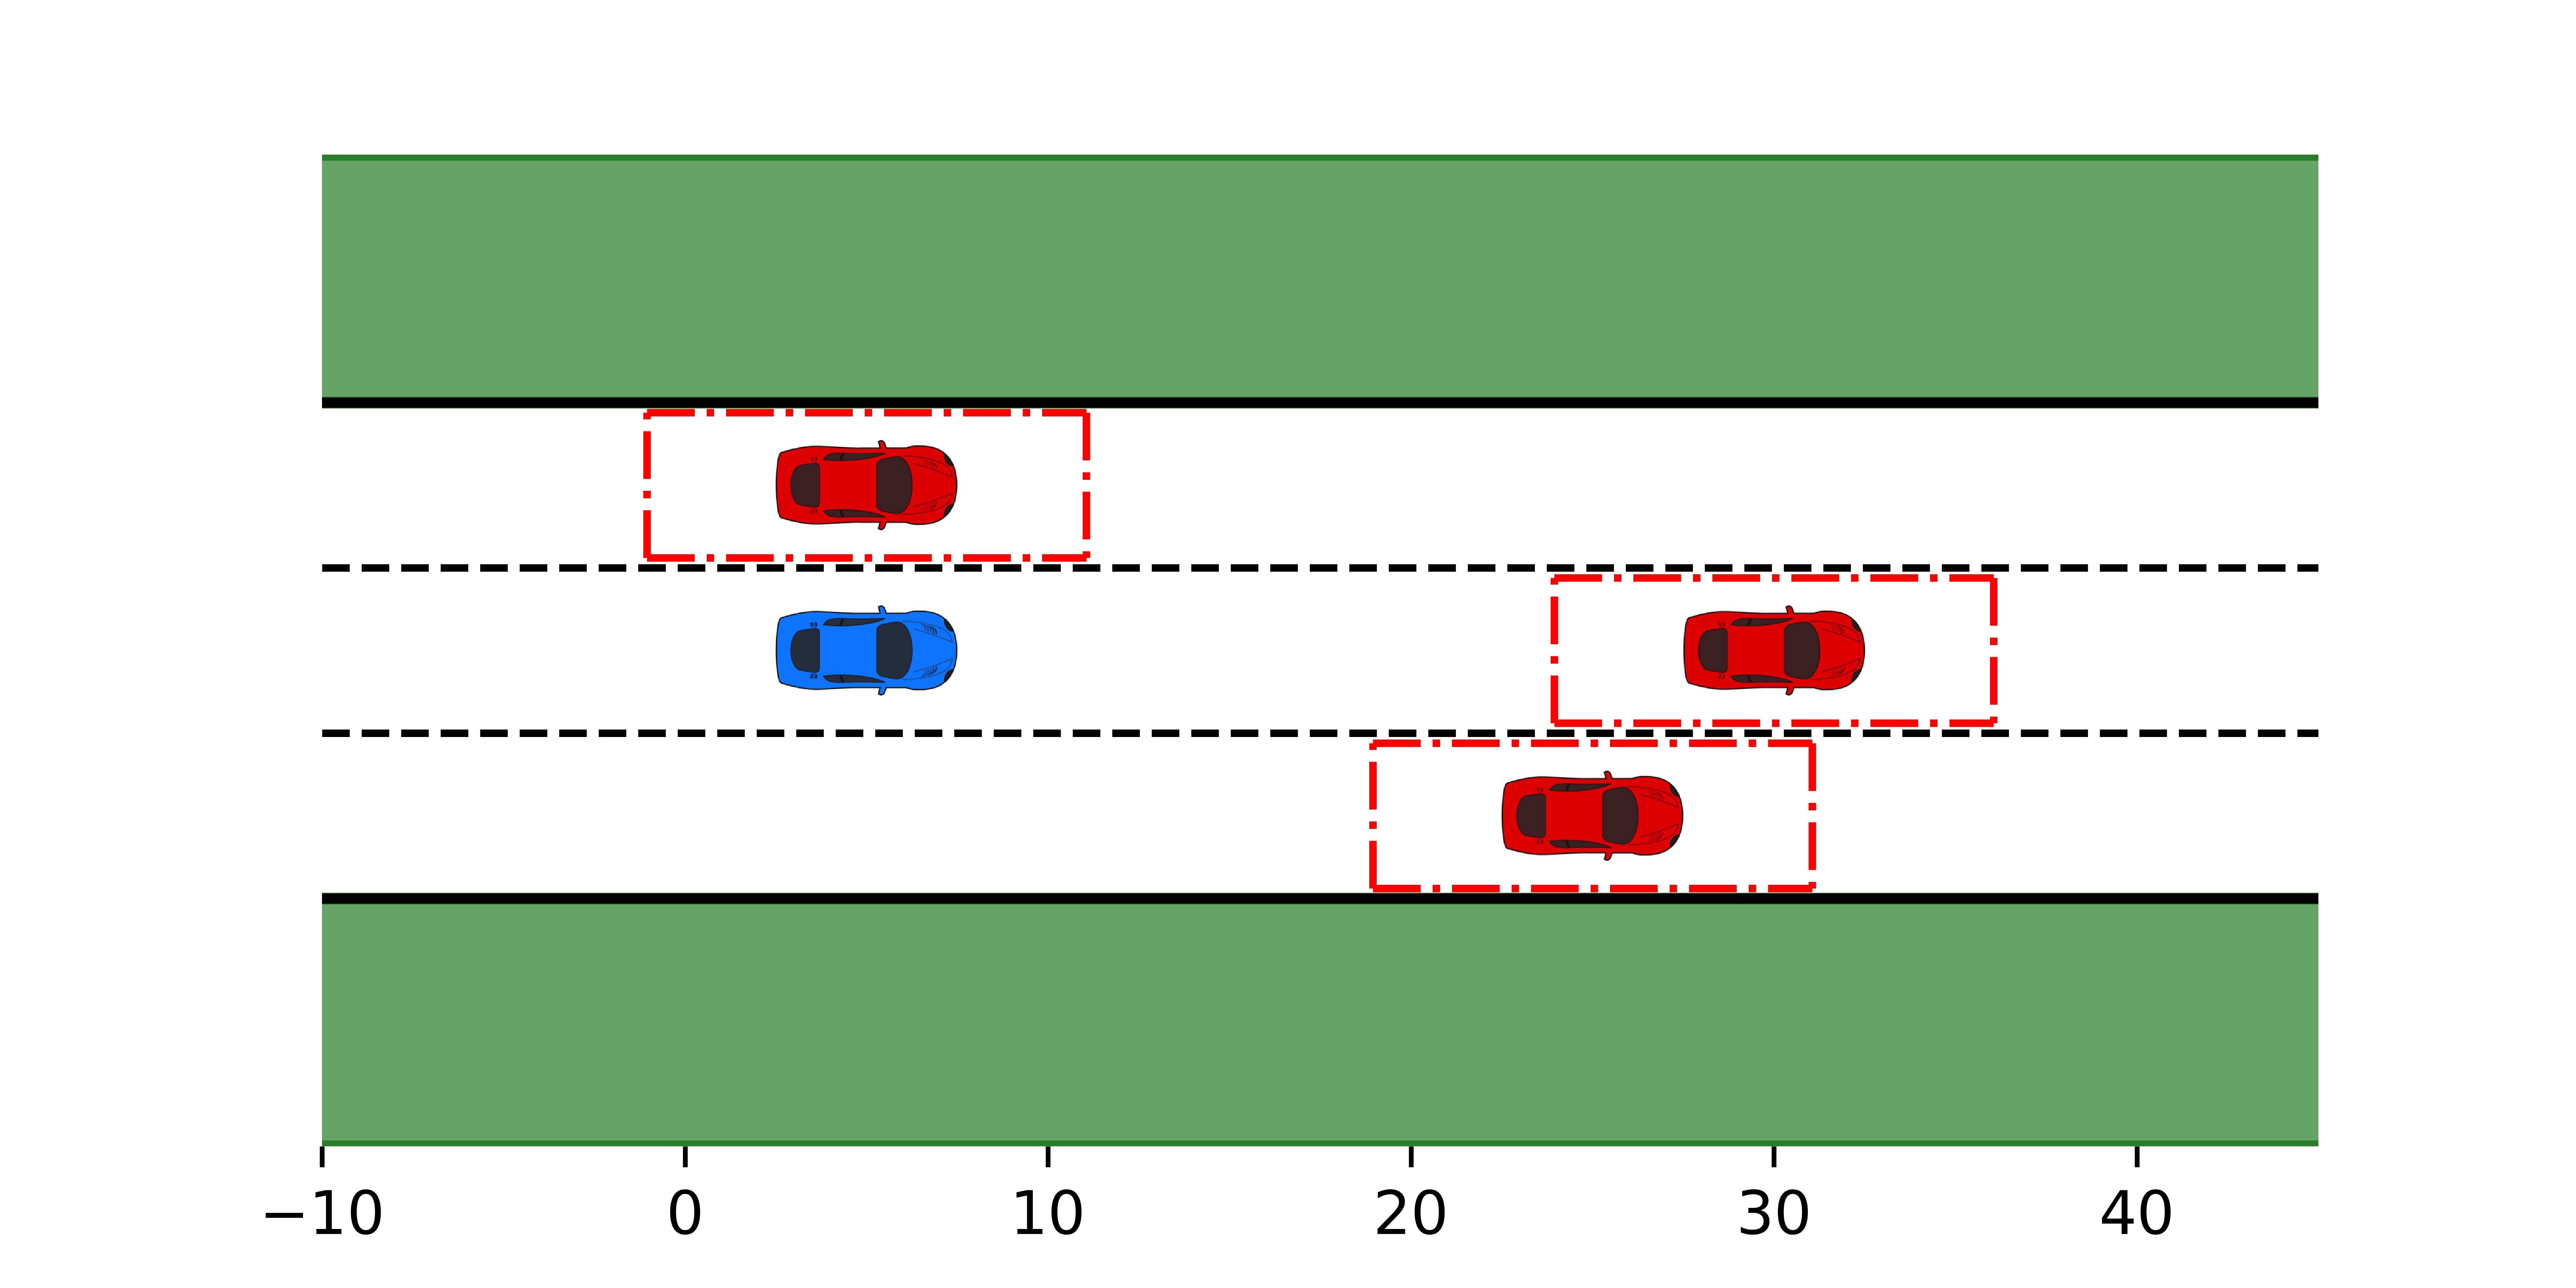
\includegraphics[clip, trim = {1.5cm 0.25cm 1.5cm 0.25cm}]{plot_adp0.jpg}};
			\node (agg1)[left = 1cm of adp1, minimum width = 0.cm, minimum height = 0cm, inner sep = 0pt]{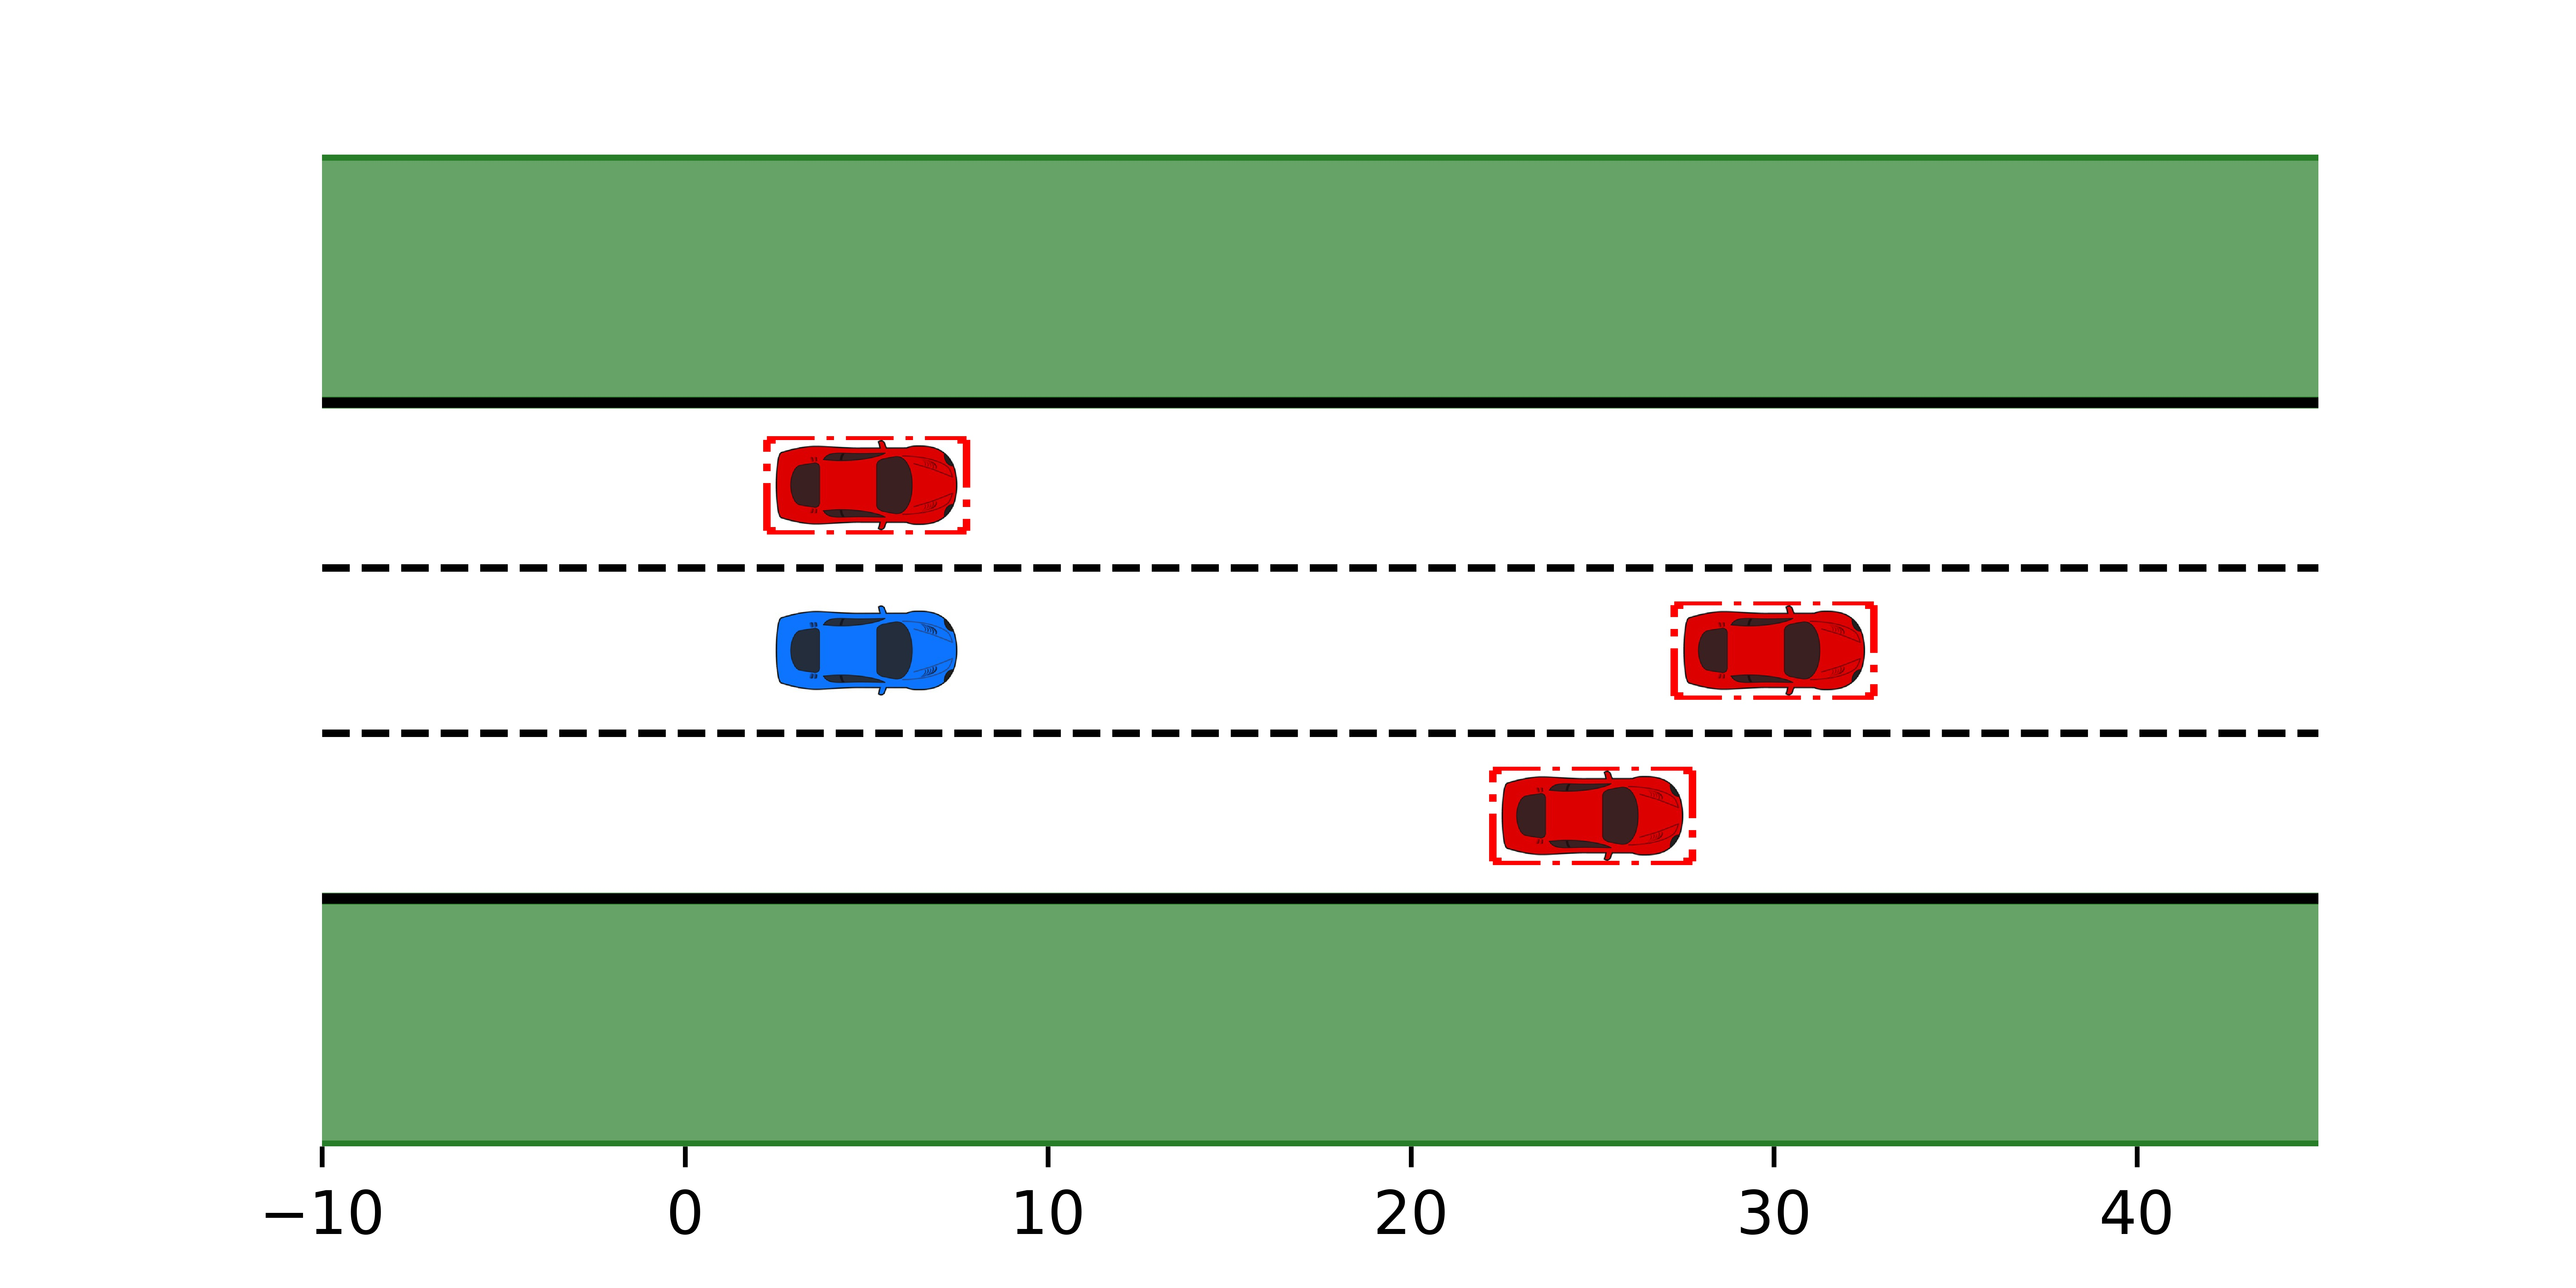
\includegraphics[clip, trim = {1.5cm 0.25cm 1.5cm 0.25cm}]{plot_agg0.jpg}};
			\node (con1)[ right = 1cm of adp1, minimum width = 0.cm, minimum height = 0cm, inner sep = 0pt]{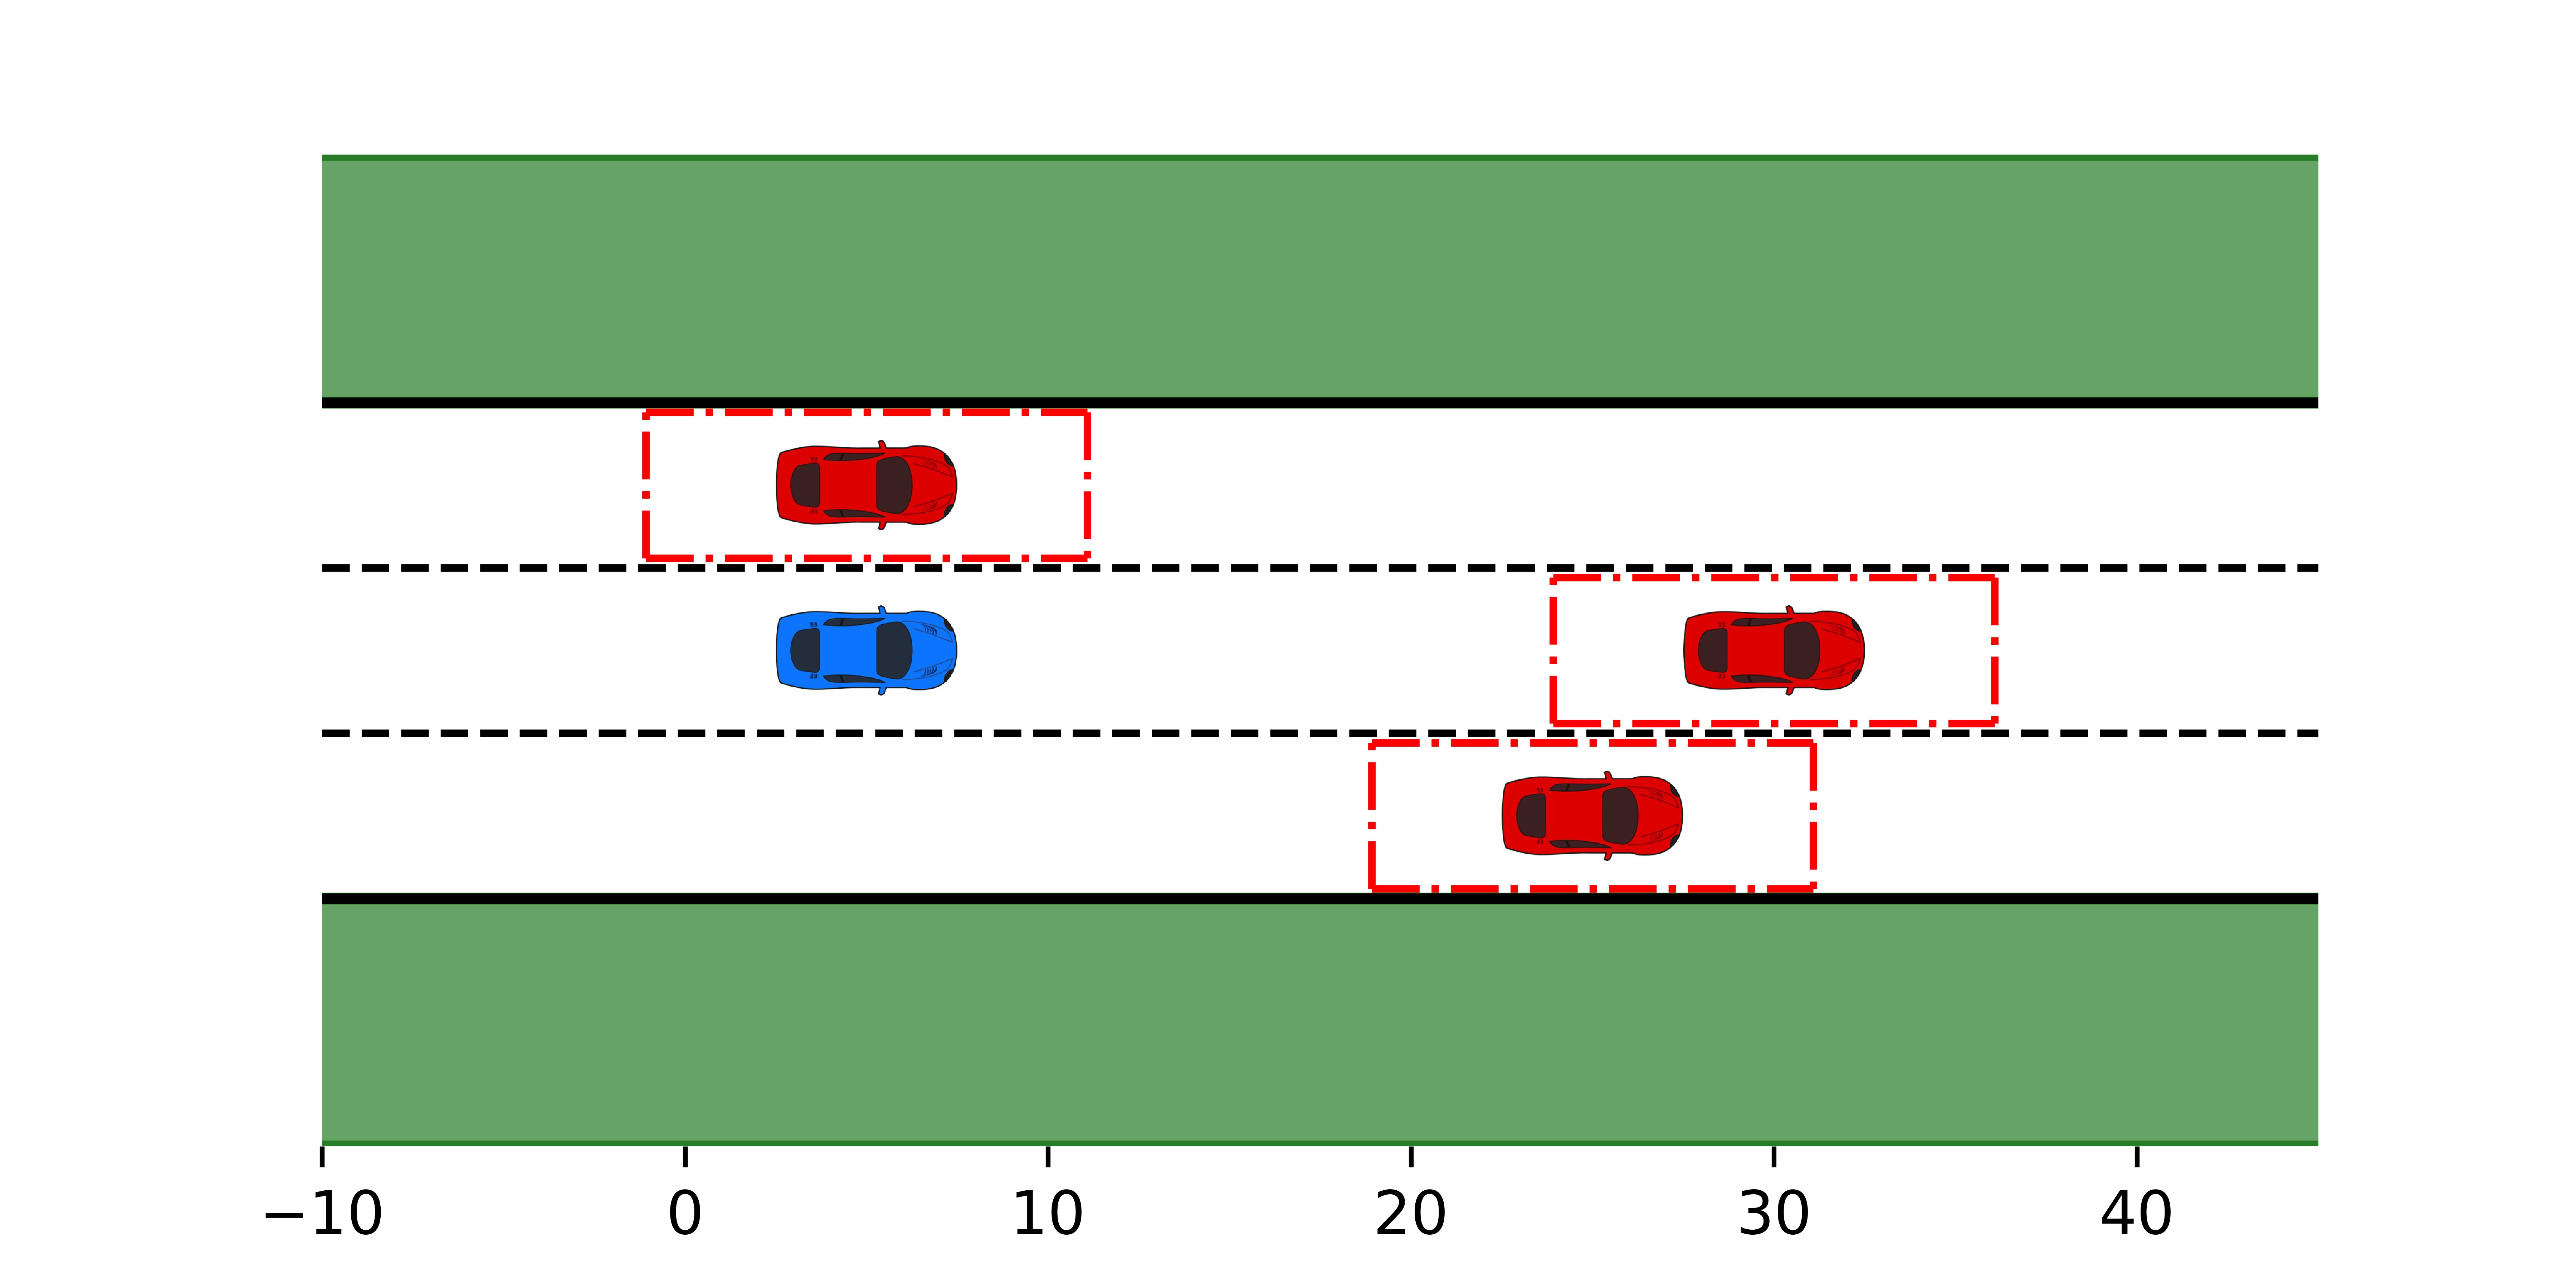
\includegraphics[clip, trim = {1.5cm 0.25cm 1.5cm 0.25cm}]{plot_con0.jpg}};
			
			
			\node (adp2)[below  = 1.cm of adp1, minimum width = 0.cm, minimum height = 0cm, inner sep = 0pt]{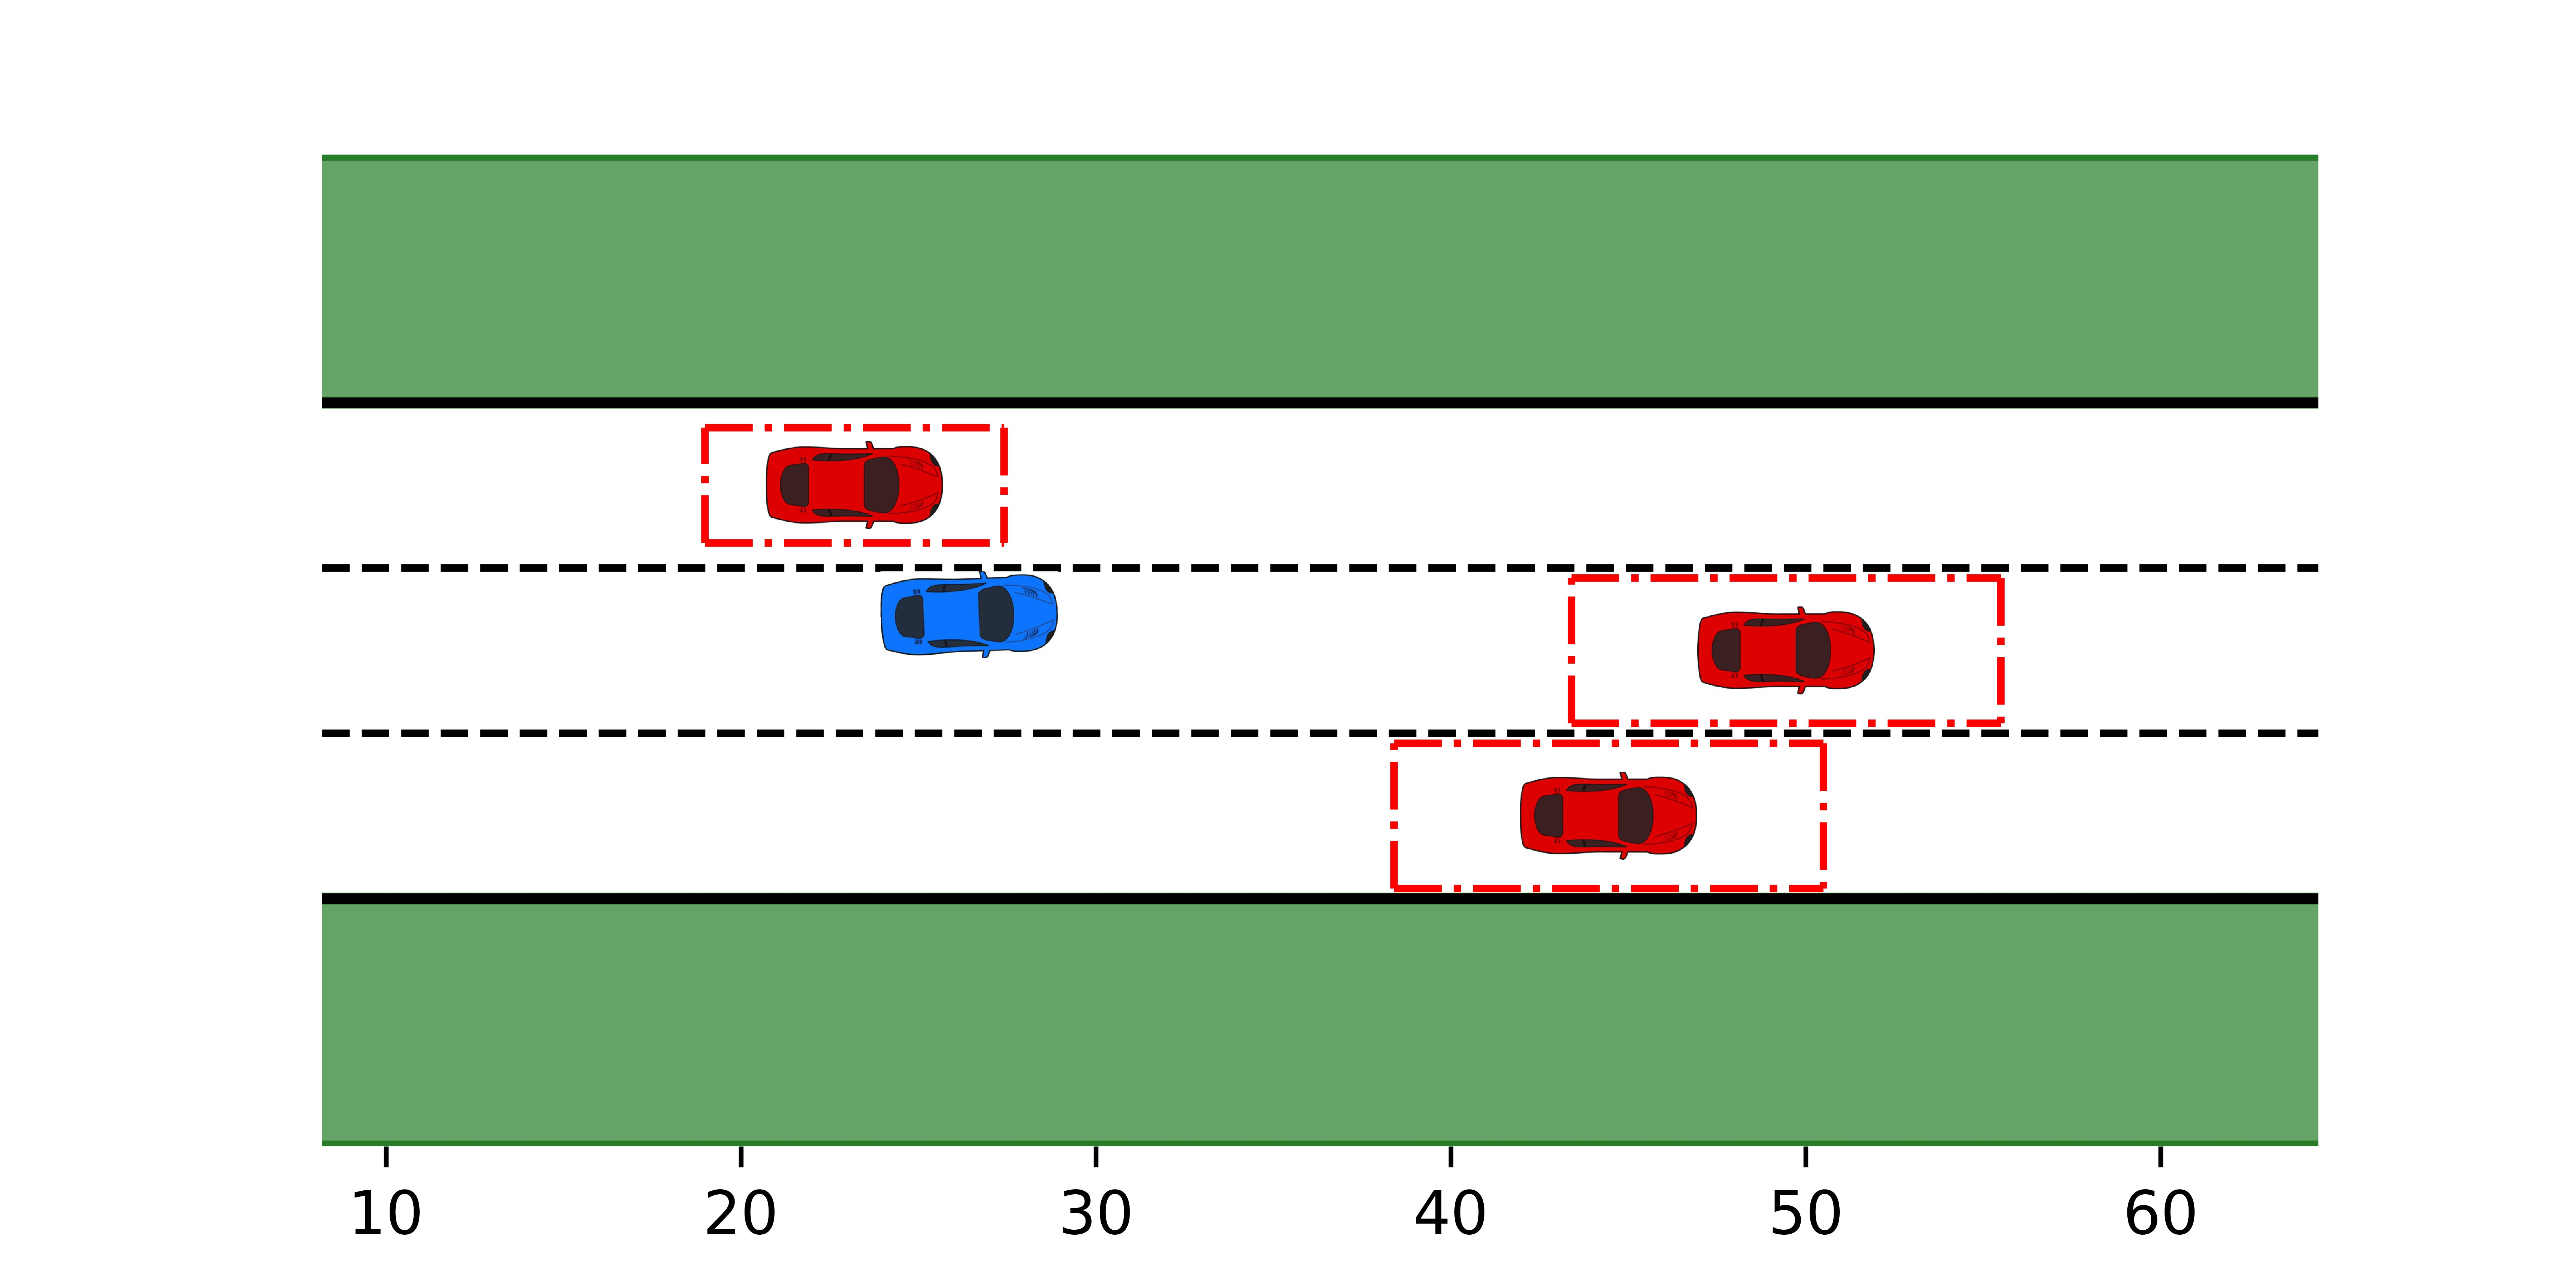
\includegraphics[clip, trim = {1.5cm 0.25cm 1.5cm 0.25cm}]{plot_adp2.jpg}};
			\node (agg2)[left = 1cm of adp2, minimum width = 0.cm, minimum height = 0cm, inner sep = 0pt]{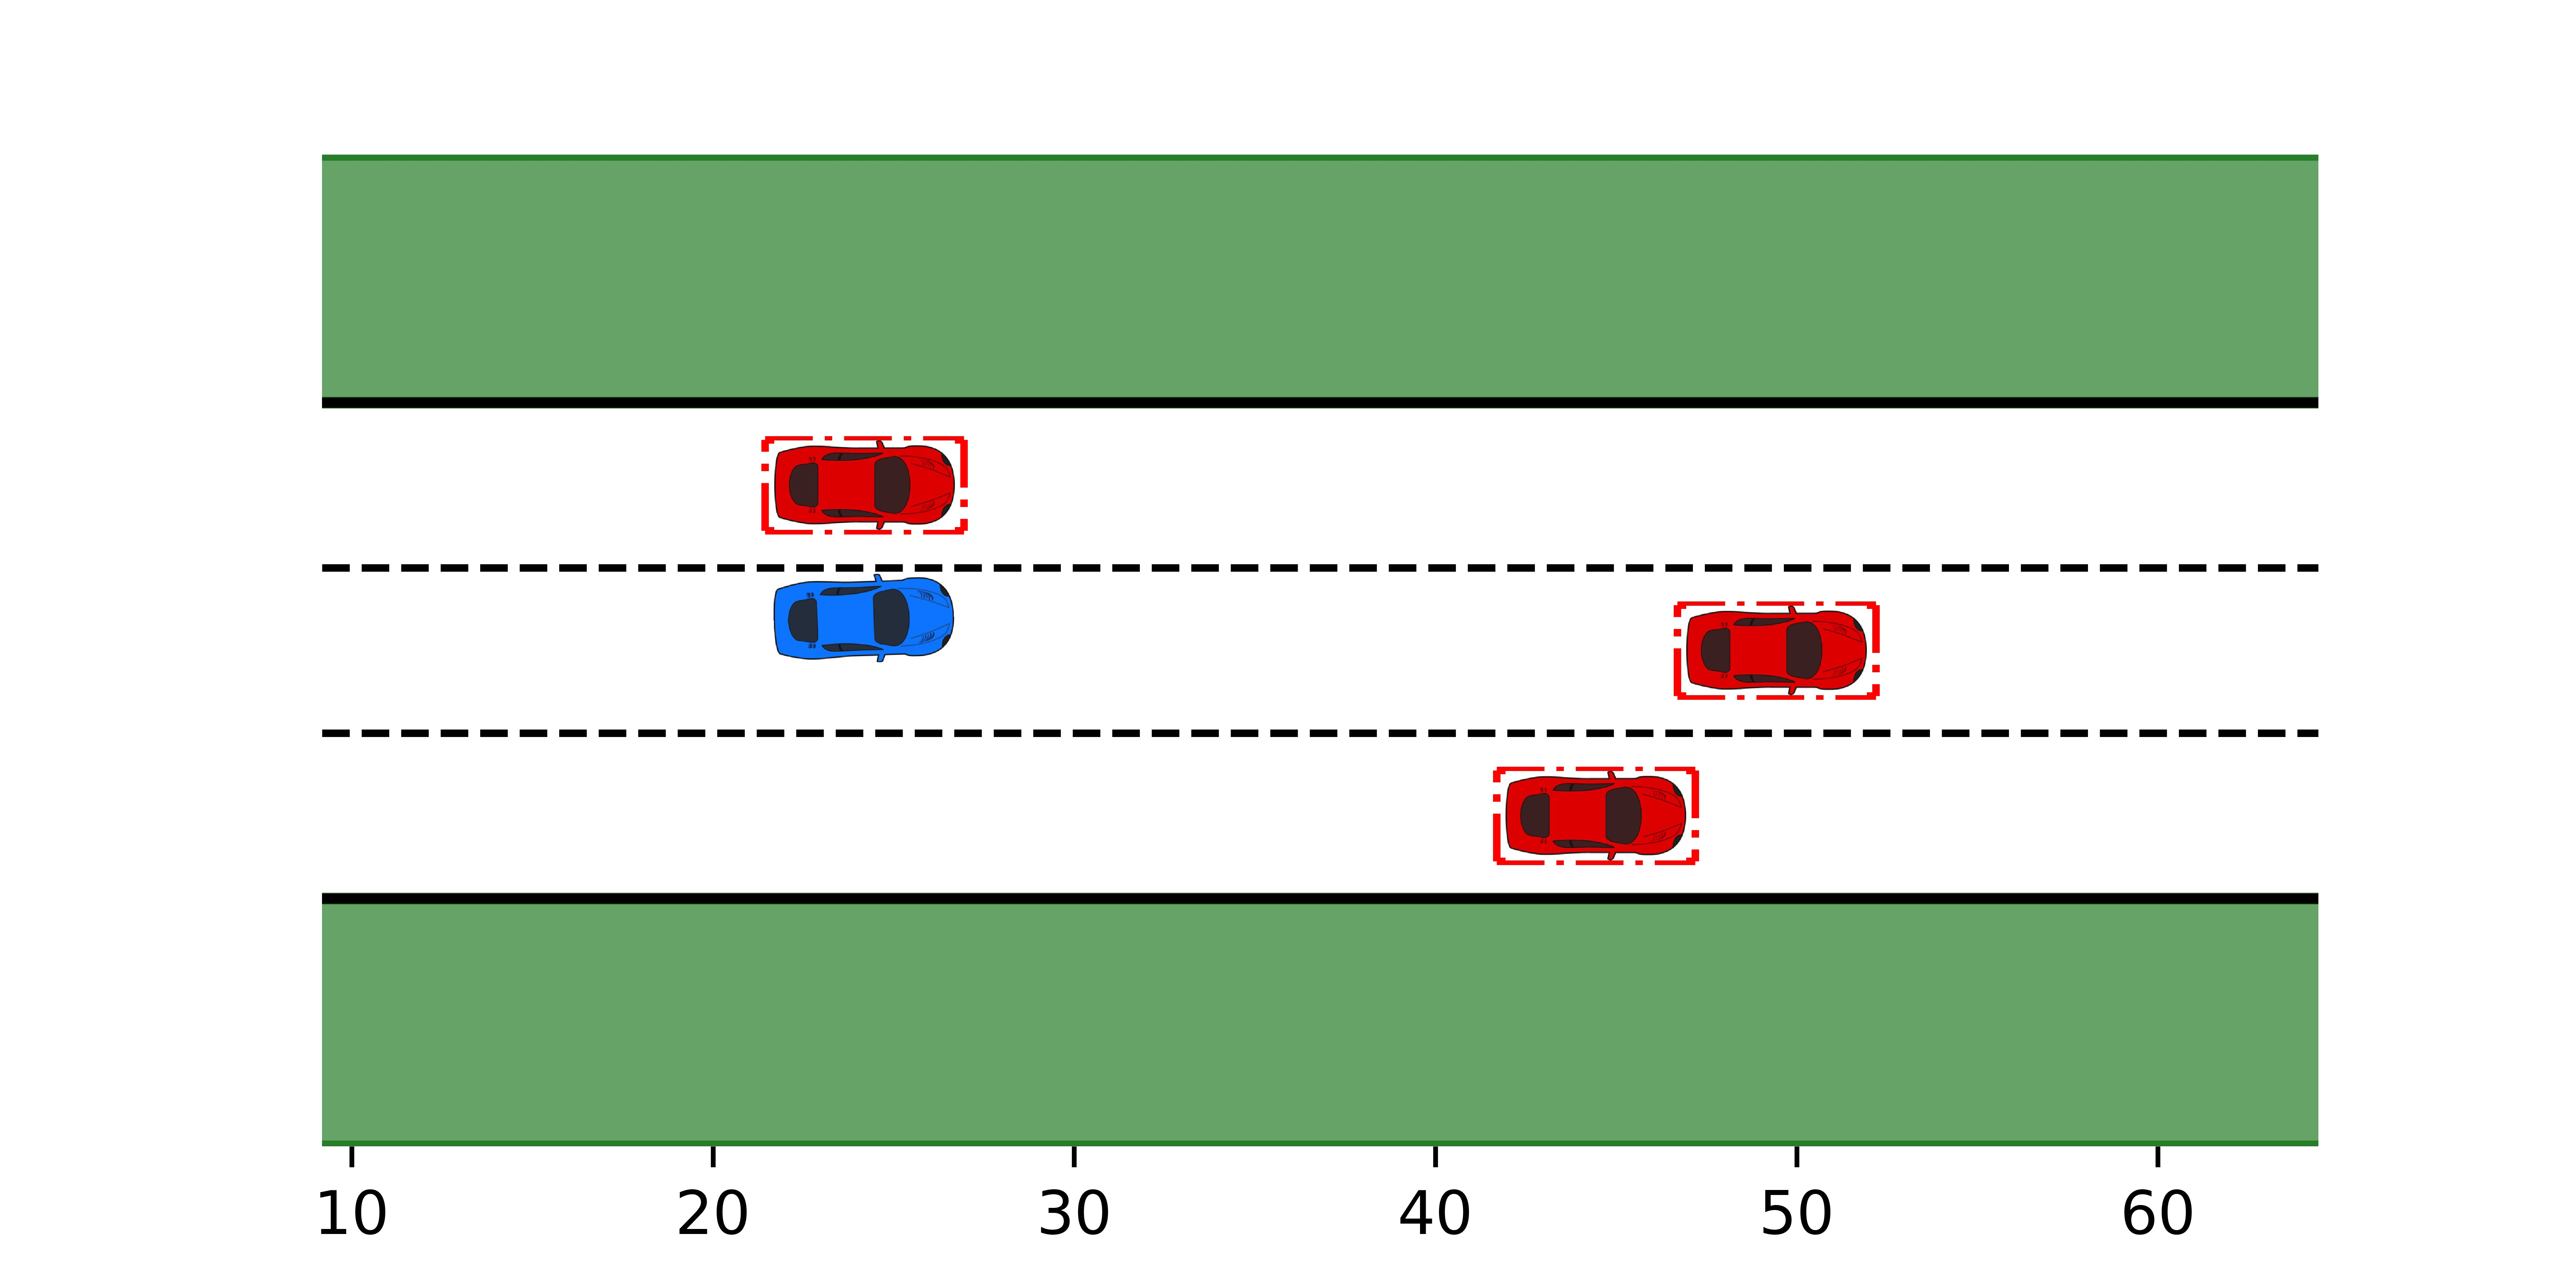
\includegraphics[clip, trim = {1.5cm 0.25cm 1.5cm 0.25cm}]{plot_agg2.jpg}};
			\node (con2)[ right = 1cm of adp2, minimum width = 0.cm, minimum height = 0cm, inner sep = 0pt]{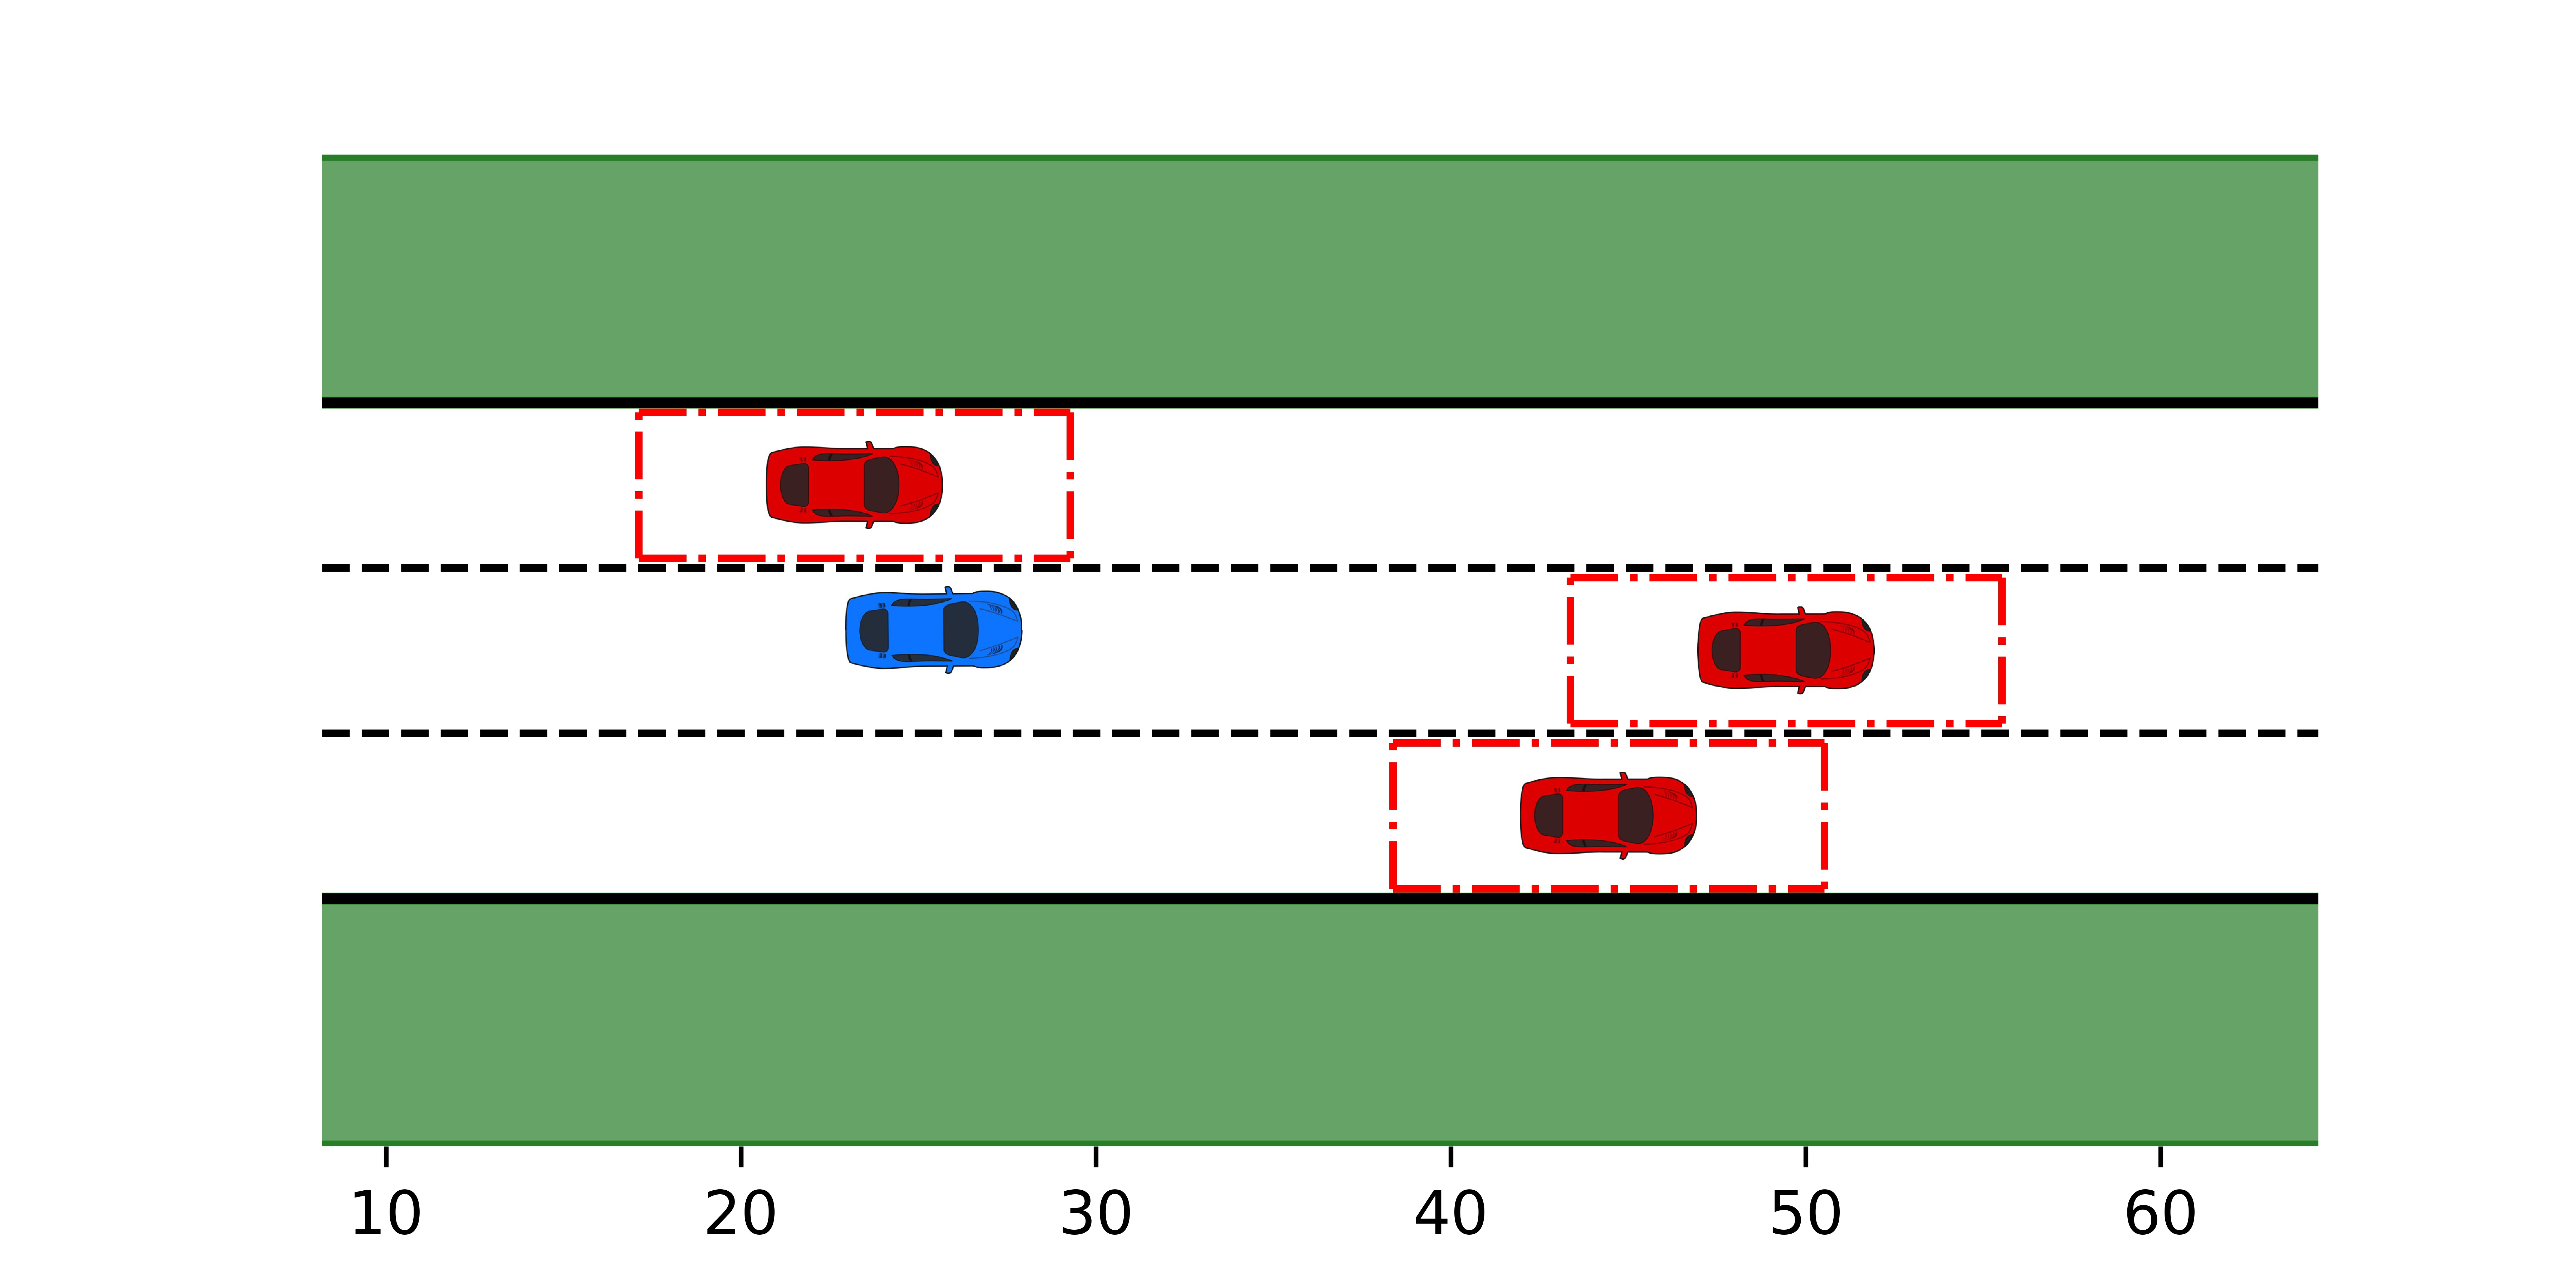
\includegraphics[clip, trim = {1.5cm 0.25cm 1.5cm 0.25cm}]{plot_con2.jpg}};
			
			
			\node (adp3)[below  = 1.cm of adp2, minimum width = 0.cm, minimum height = 0cm, inner sep = 0pt]{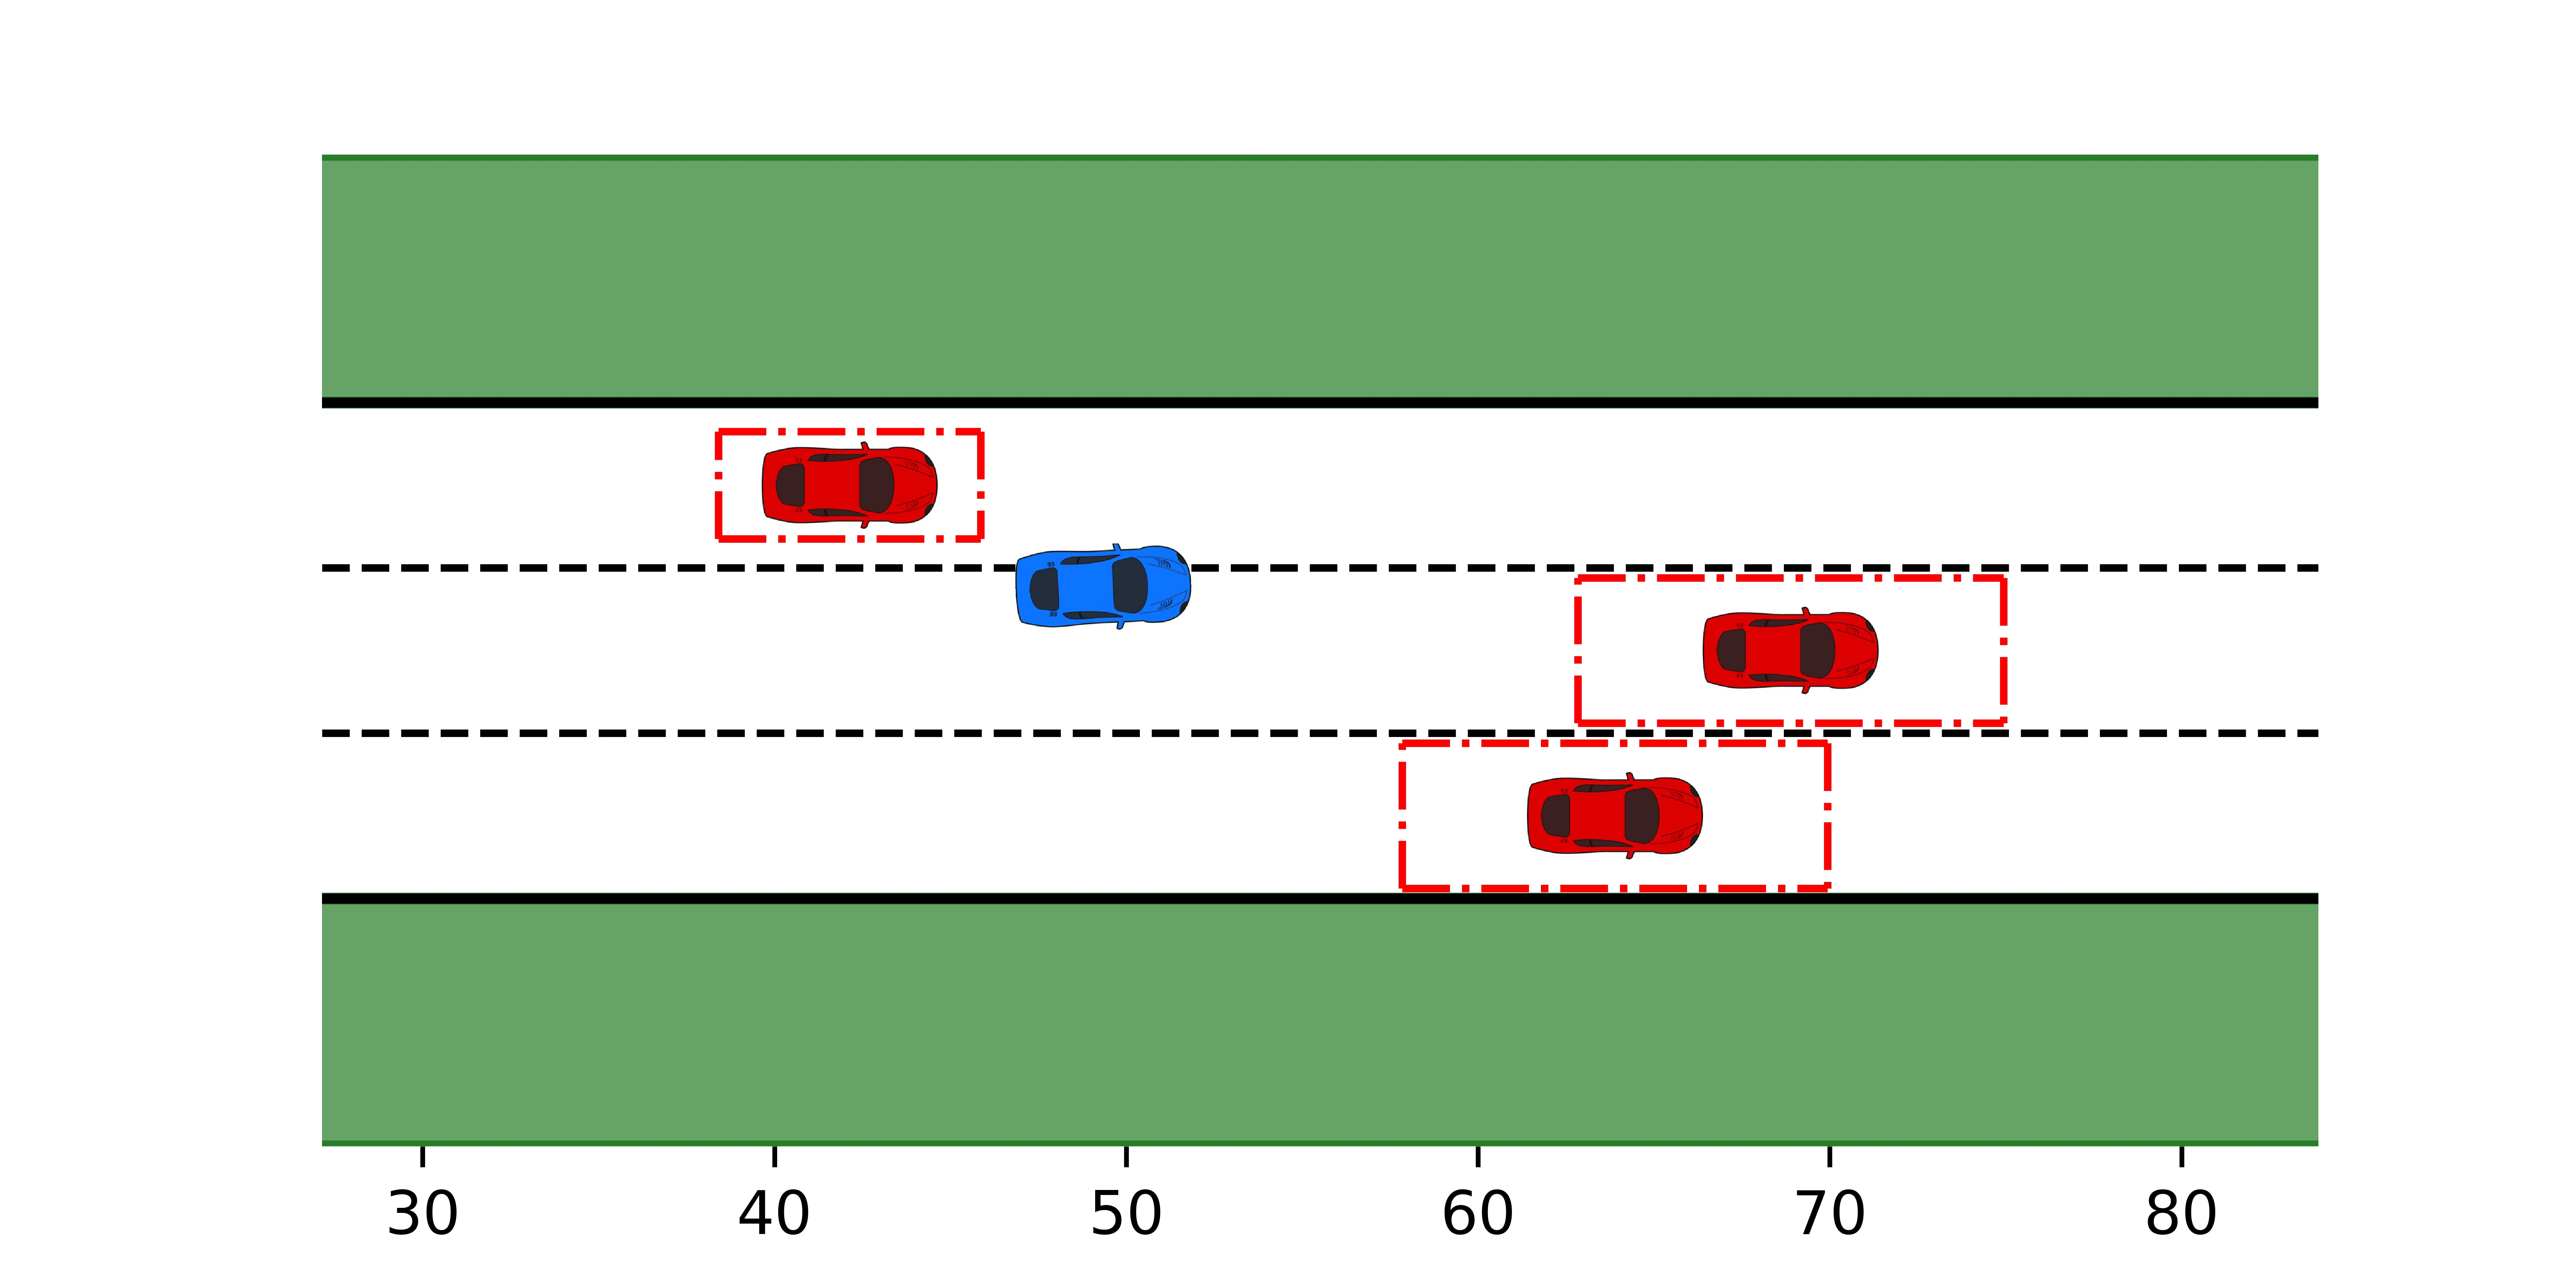
\includegraphics[clip, trim = {1.5cm 0.25cm 1.5cm 0.25cm}]{plot_adp4.jpg}};
			\node (agg3)[left = 1cm of adp3, minimum width = 0.cm, minimum height = 0cm, inner sep = 0pt]{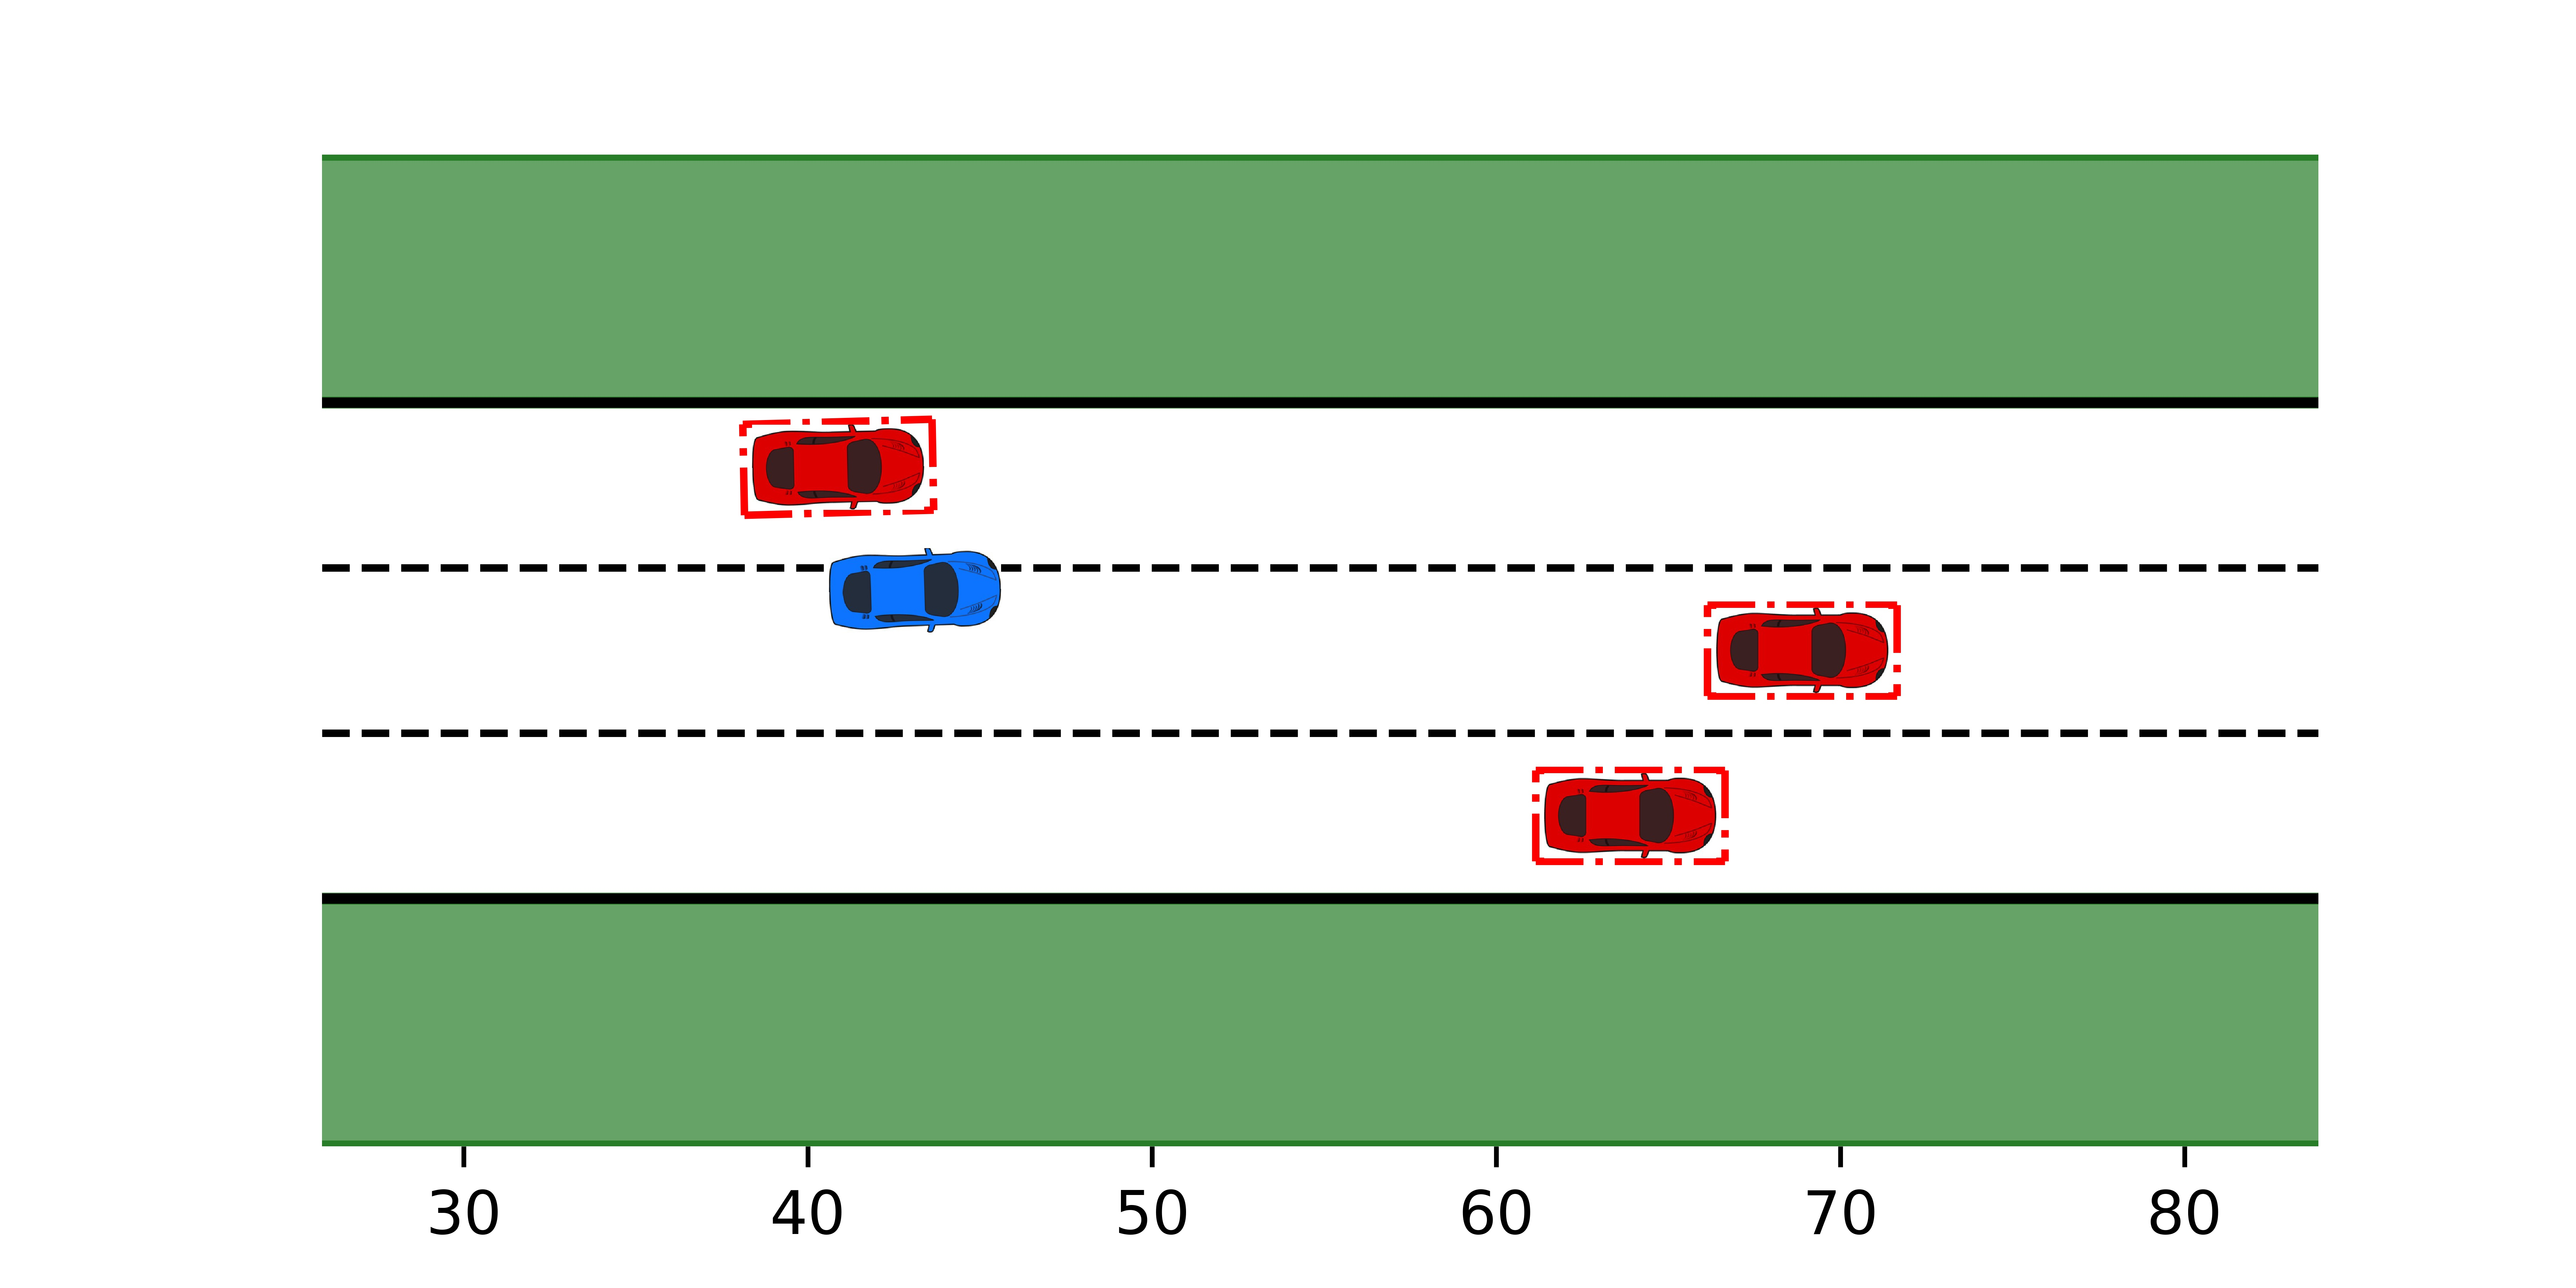
\includegraphics[clip, trim = {1.5cm 0.25cm 1.5cm 0.25cm}]{plot_agg4.jpg}};
			\node (con3)[ right = 1cm of adp3, minimum width = 0.cm, minimum height = 0cm, inner sep = 0pt]{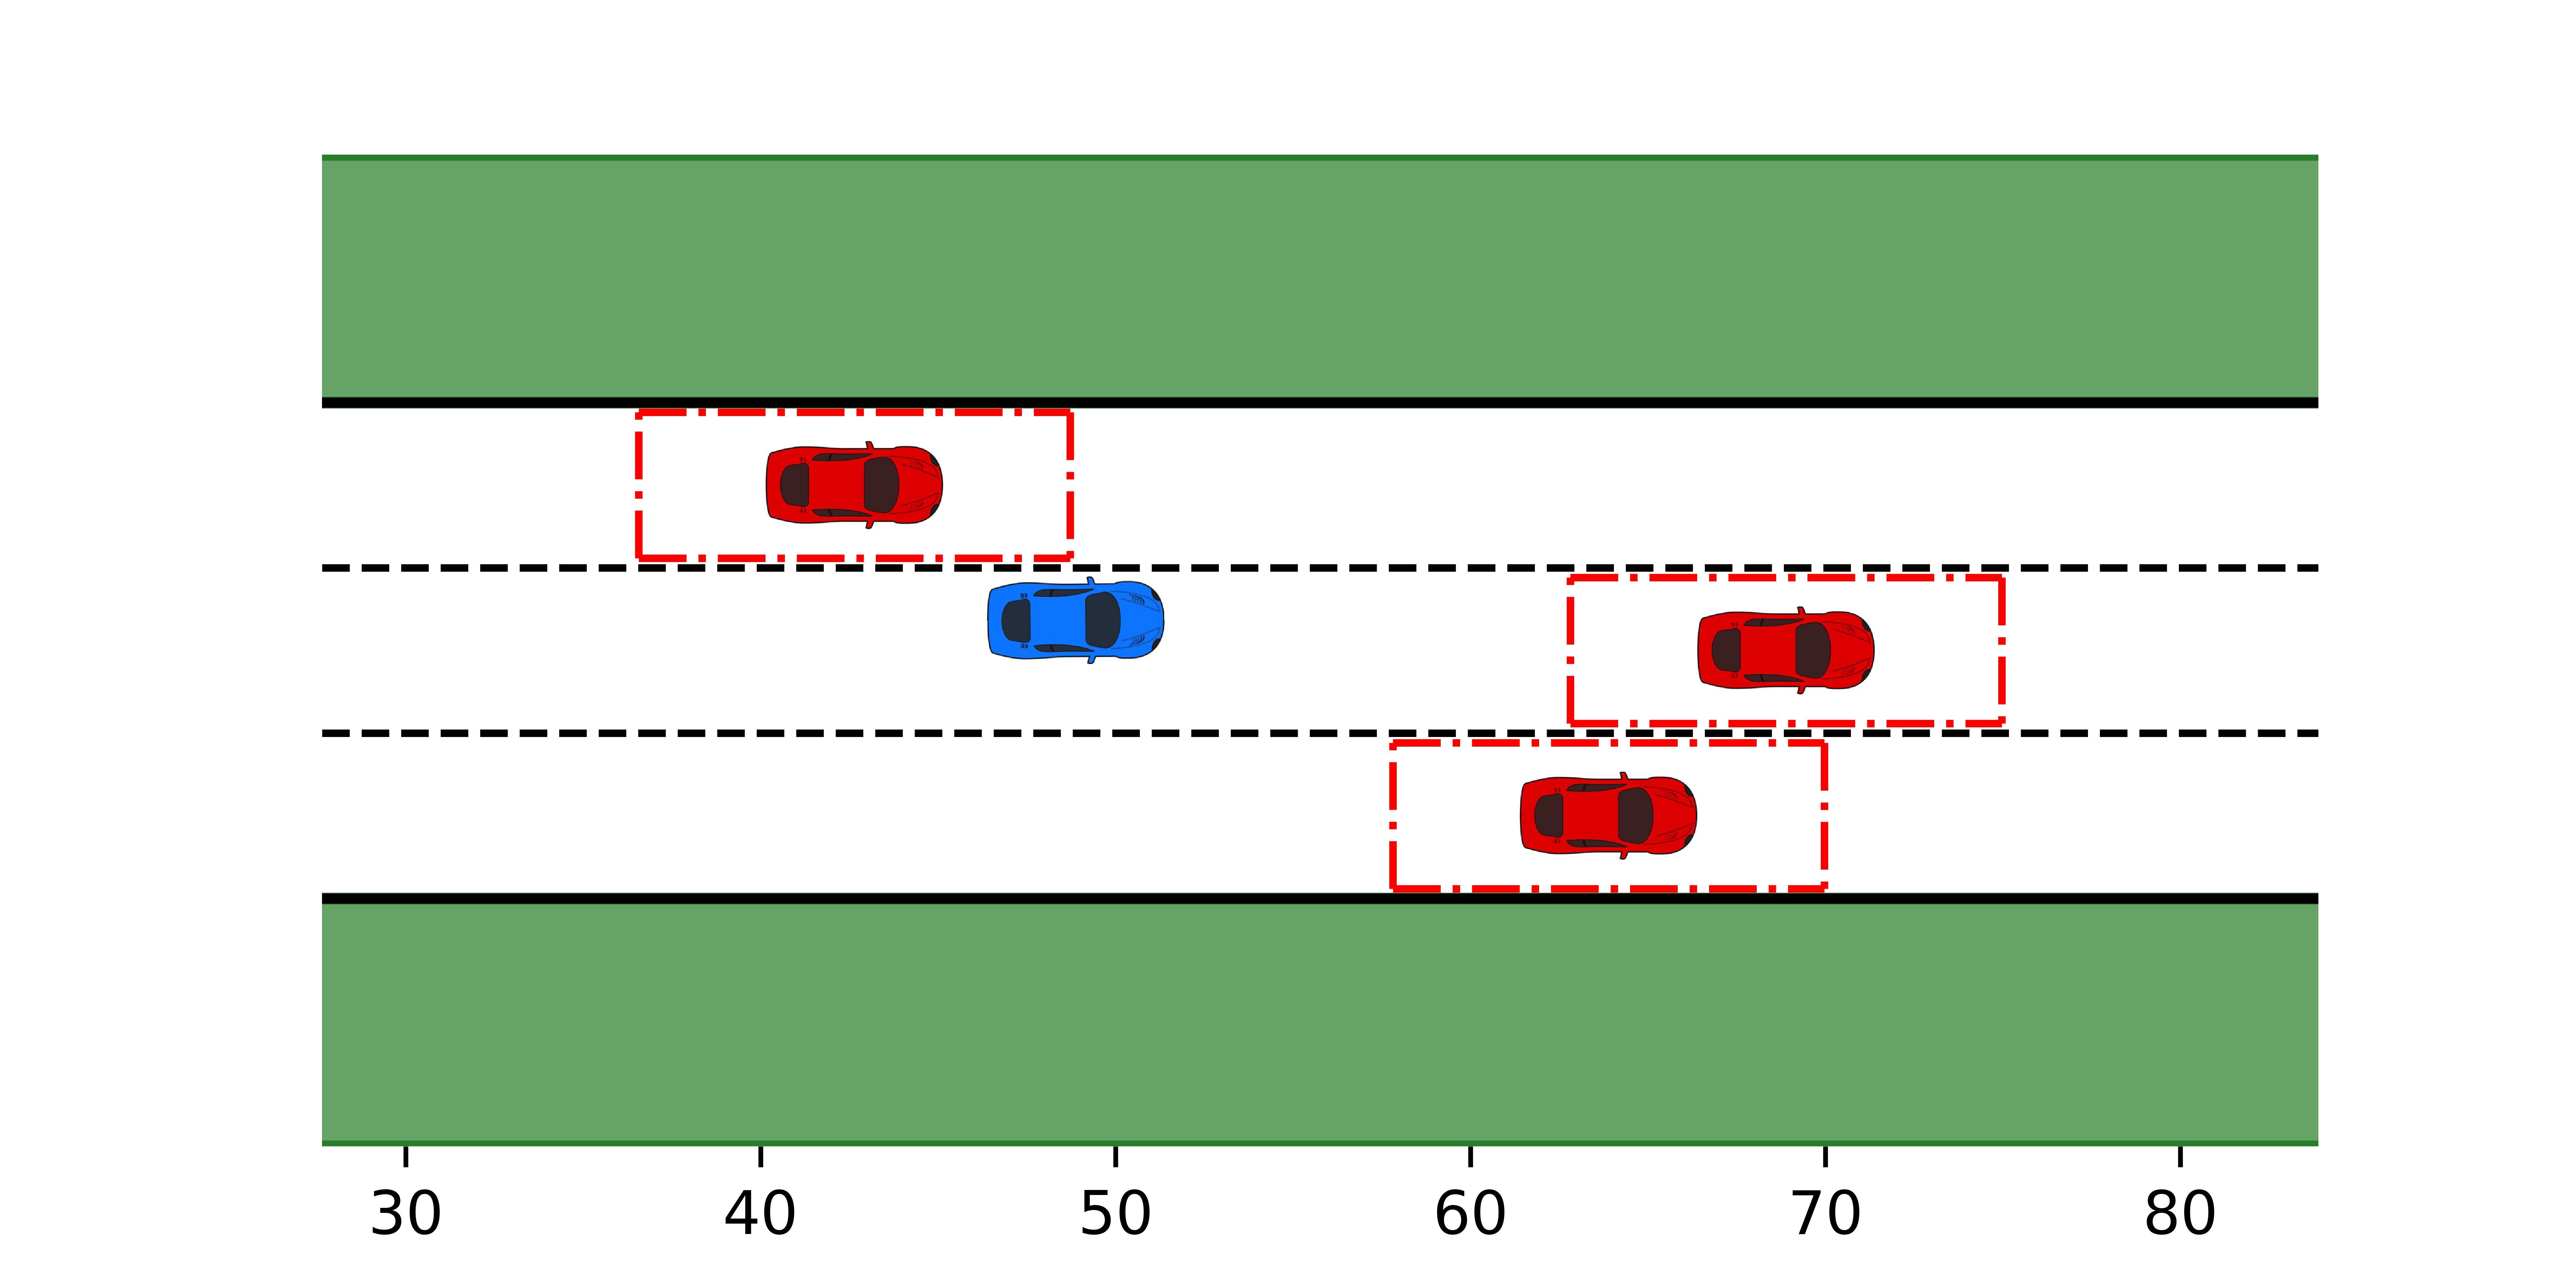
\includegraphics[clip, trim = {1.5cm 0.25cm 1.5cm 0.25cm}]{plot_con4.jpg}};
			
			
			\node (adp4)[below  = 1.cm of adp3, minimum width = 0.cm, minimum height = 0cm, inner sep = 0pt]{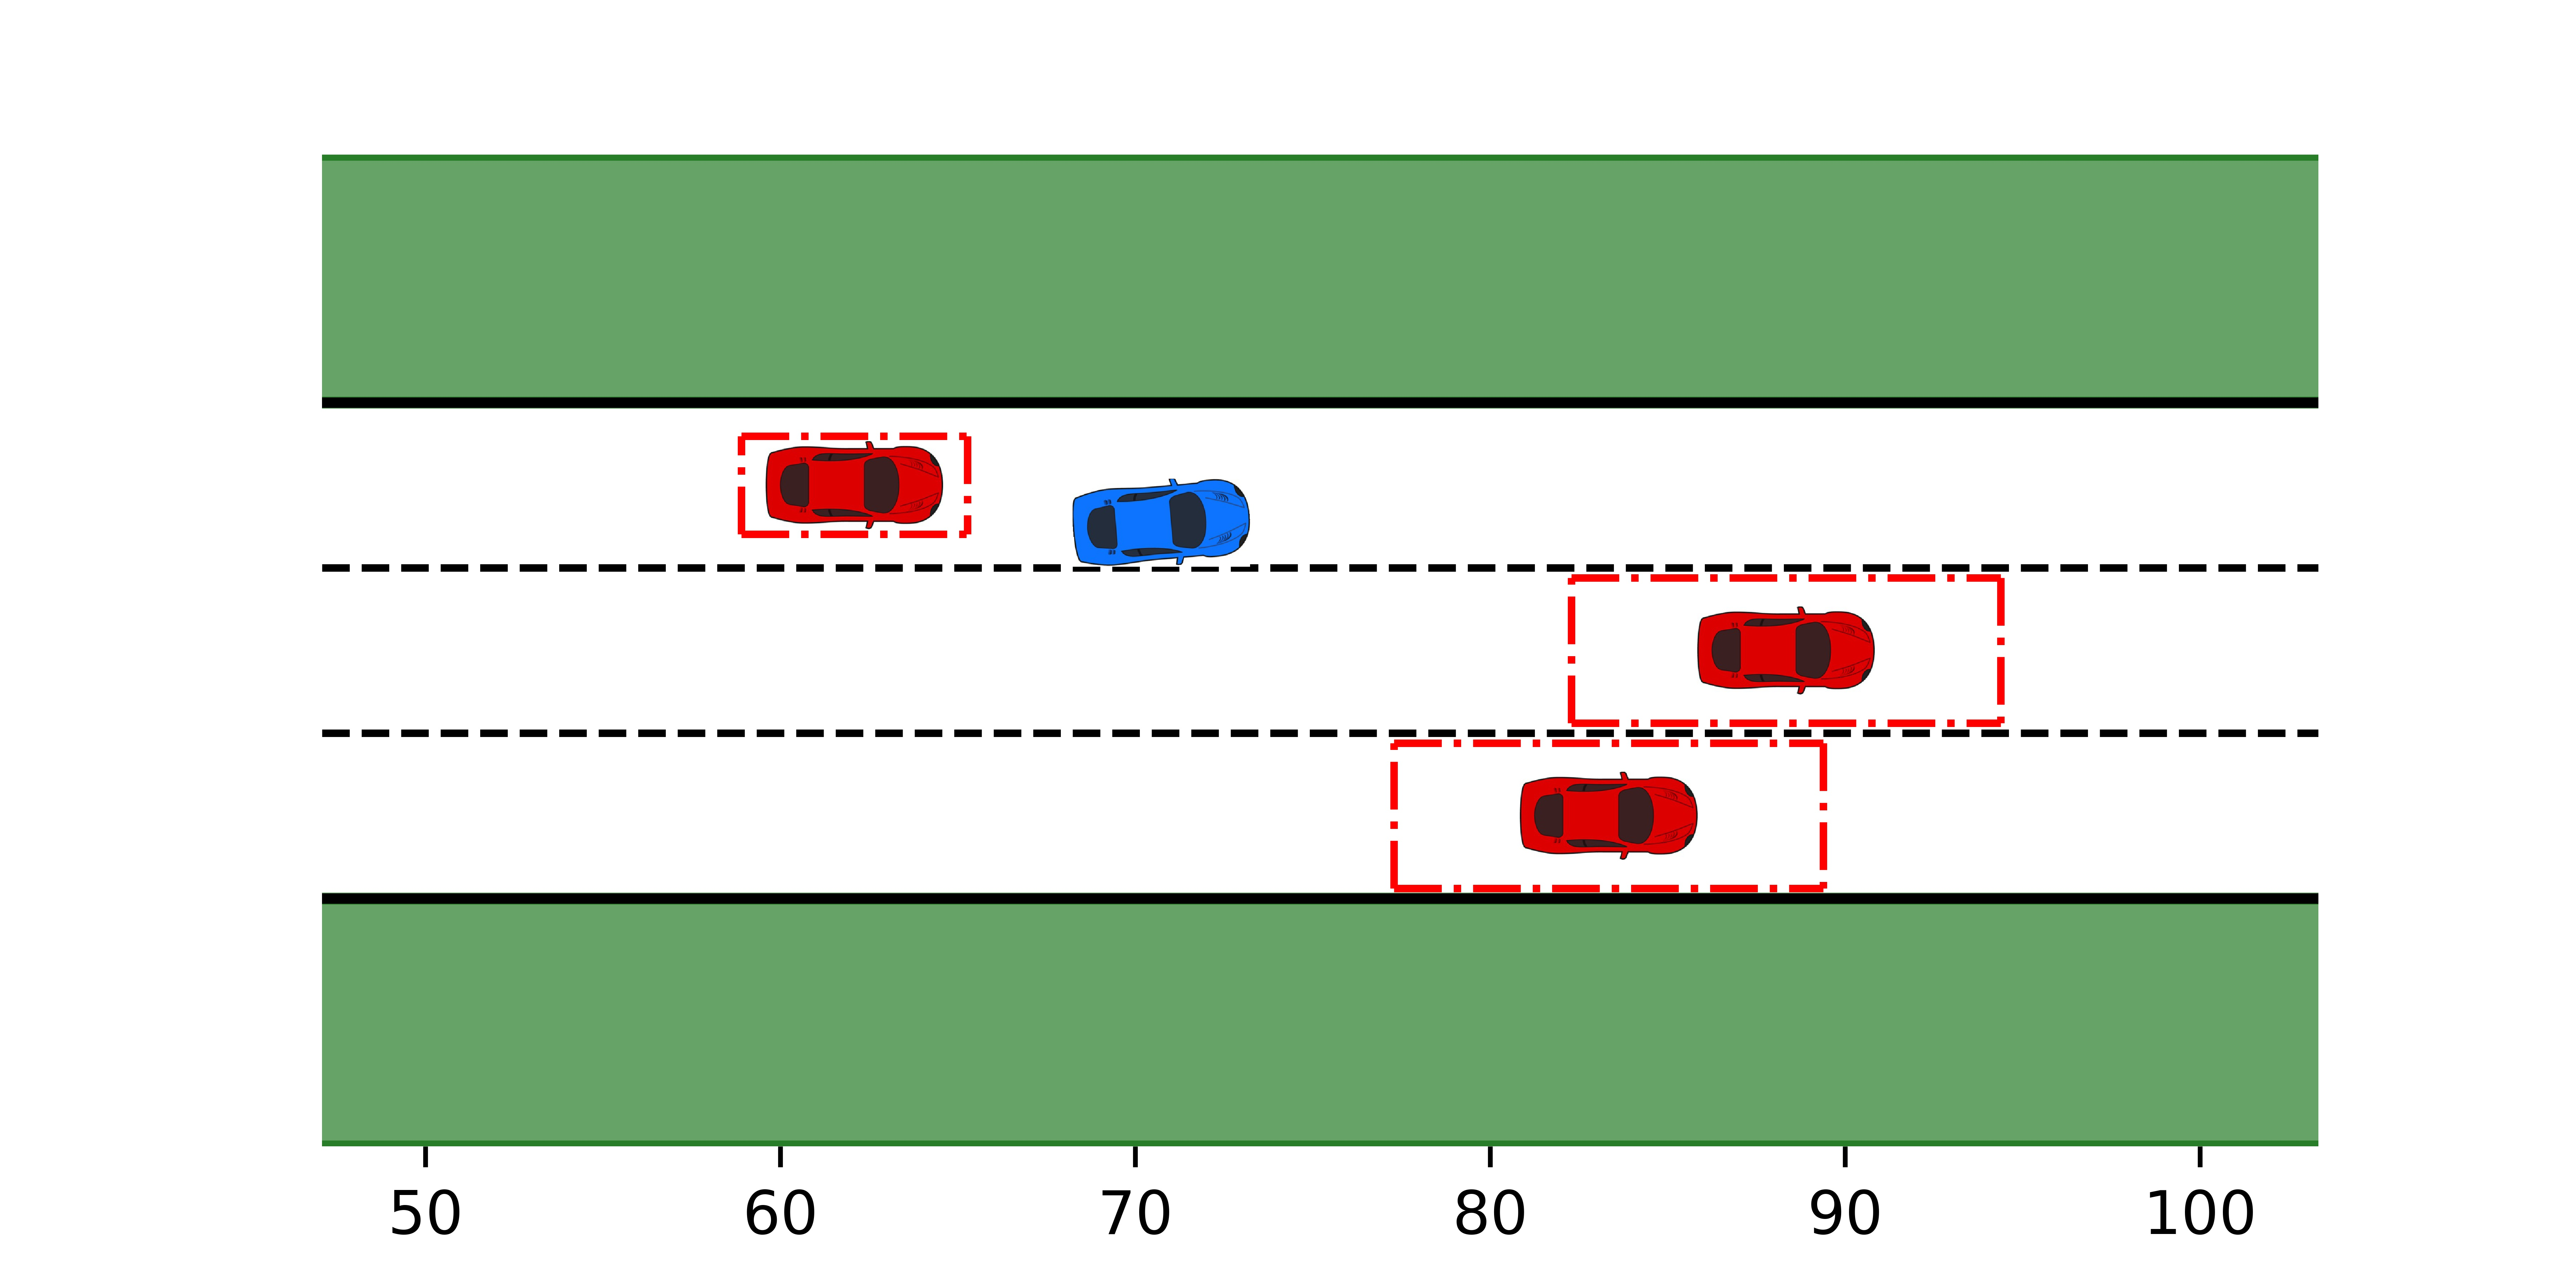
\includegraphics[clip, trim = {1.5cm 0.25cm 1.5cm 0.25cm}]{plot_adp6.jpg}};
			\node (agg4)[left = 1cm of adp4, minimum width = 0.cm, minimum height = 0cm, inner sep = 0pt]{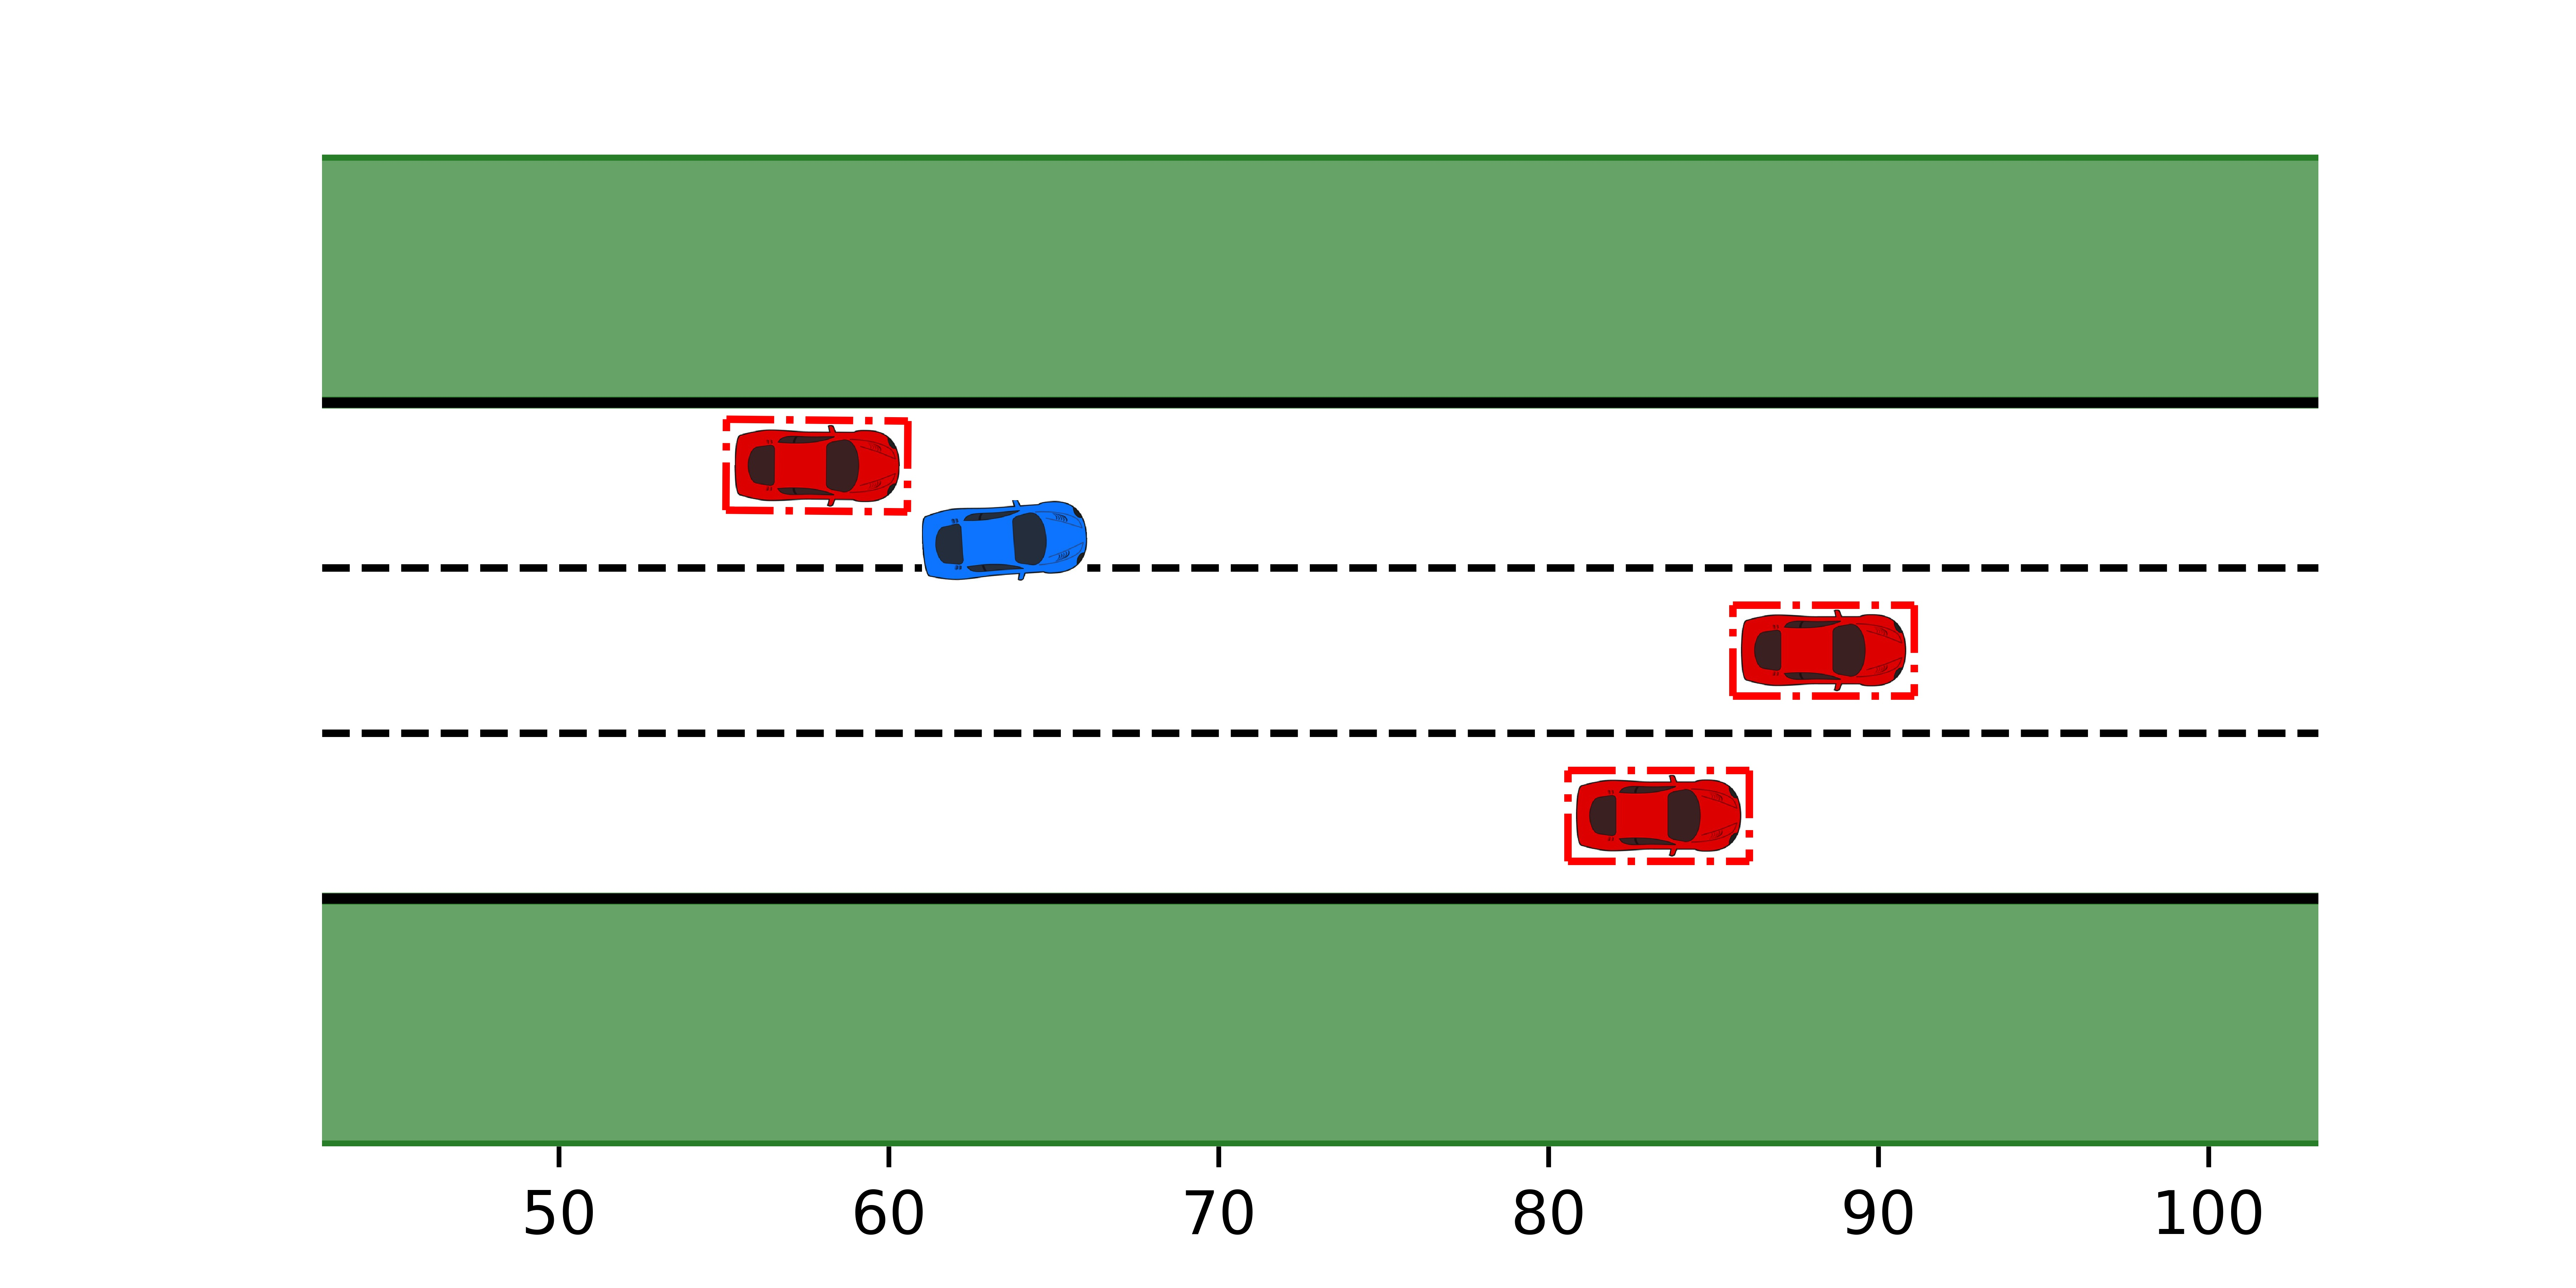
\includegraphics[clip, trim = {1.5cm 0.25cm 1.5cm 0.25cm}]{plot_agg6.jpg}};
			\node (con4)[ right = 1cm of adp4, minimum width = 0.cm, minimum height = 0cm, inner sep = 0pt]{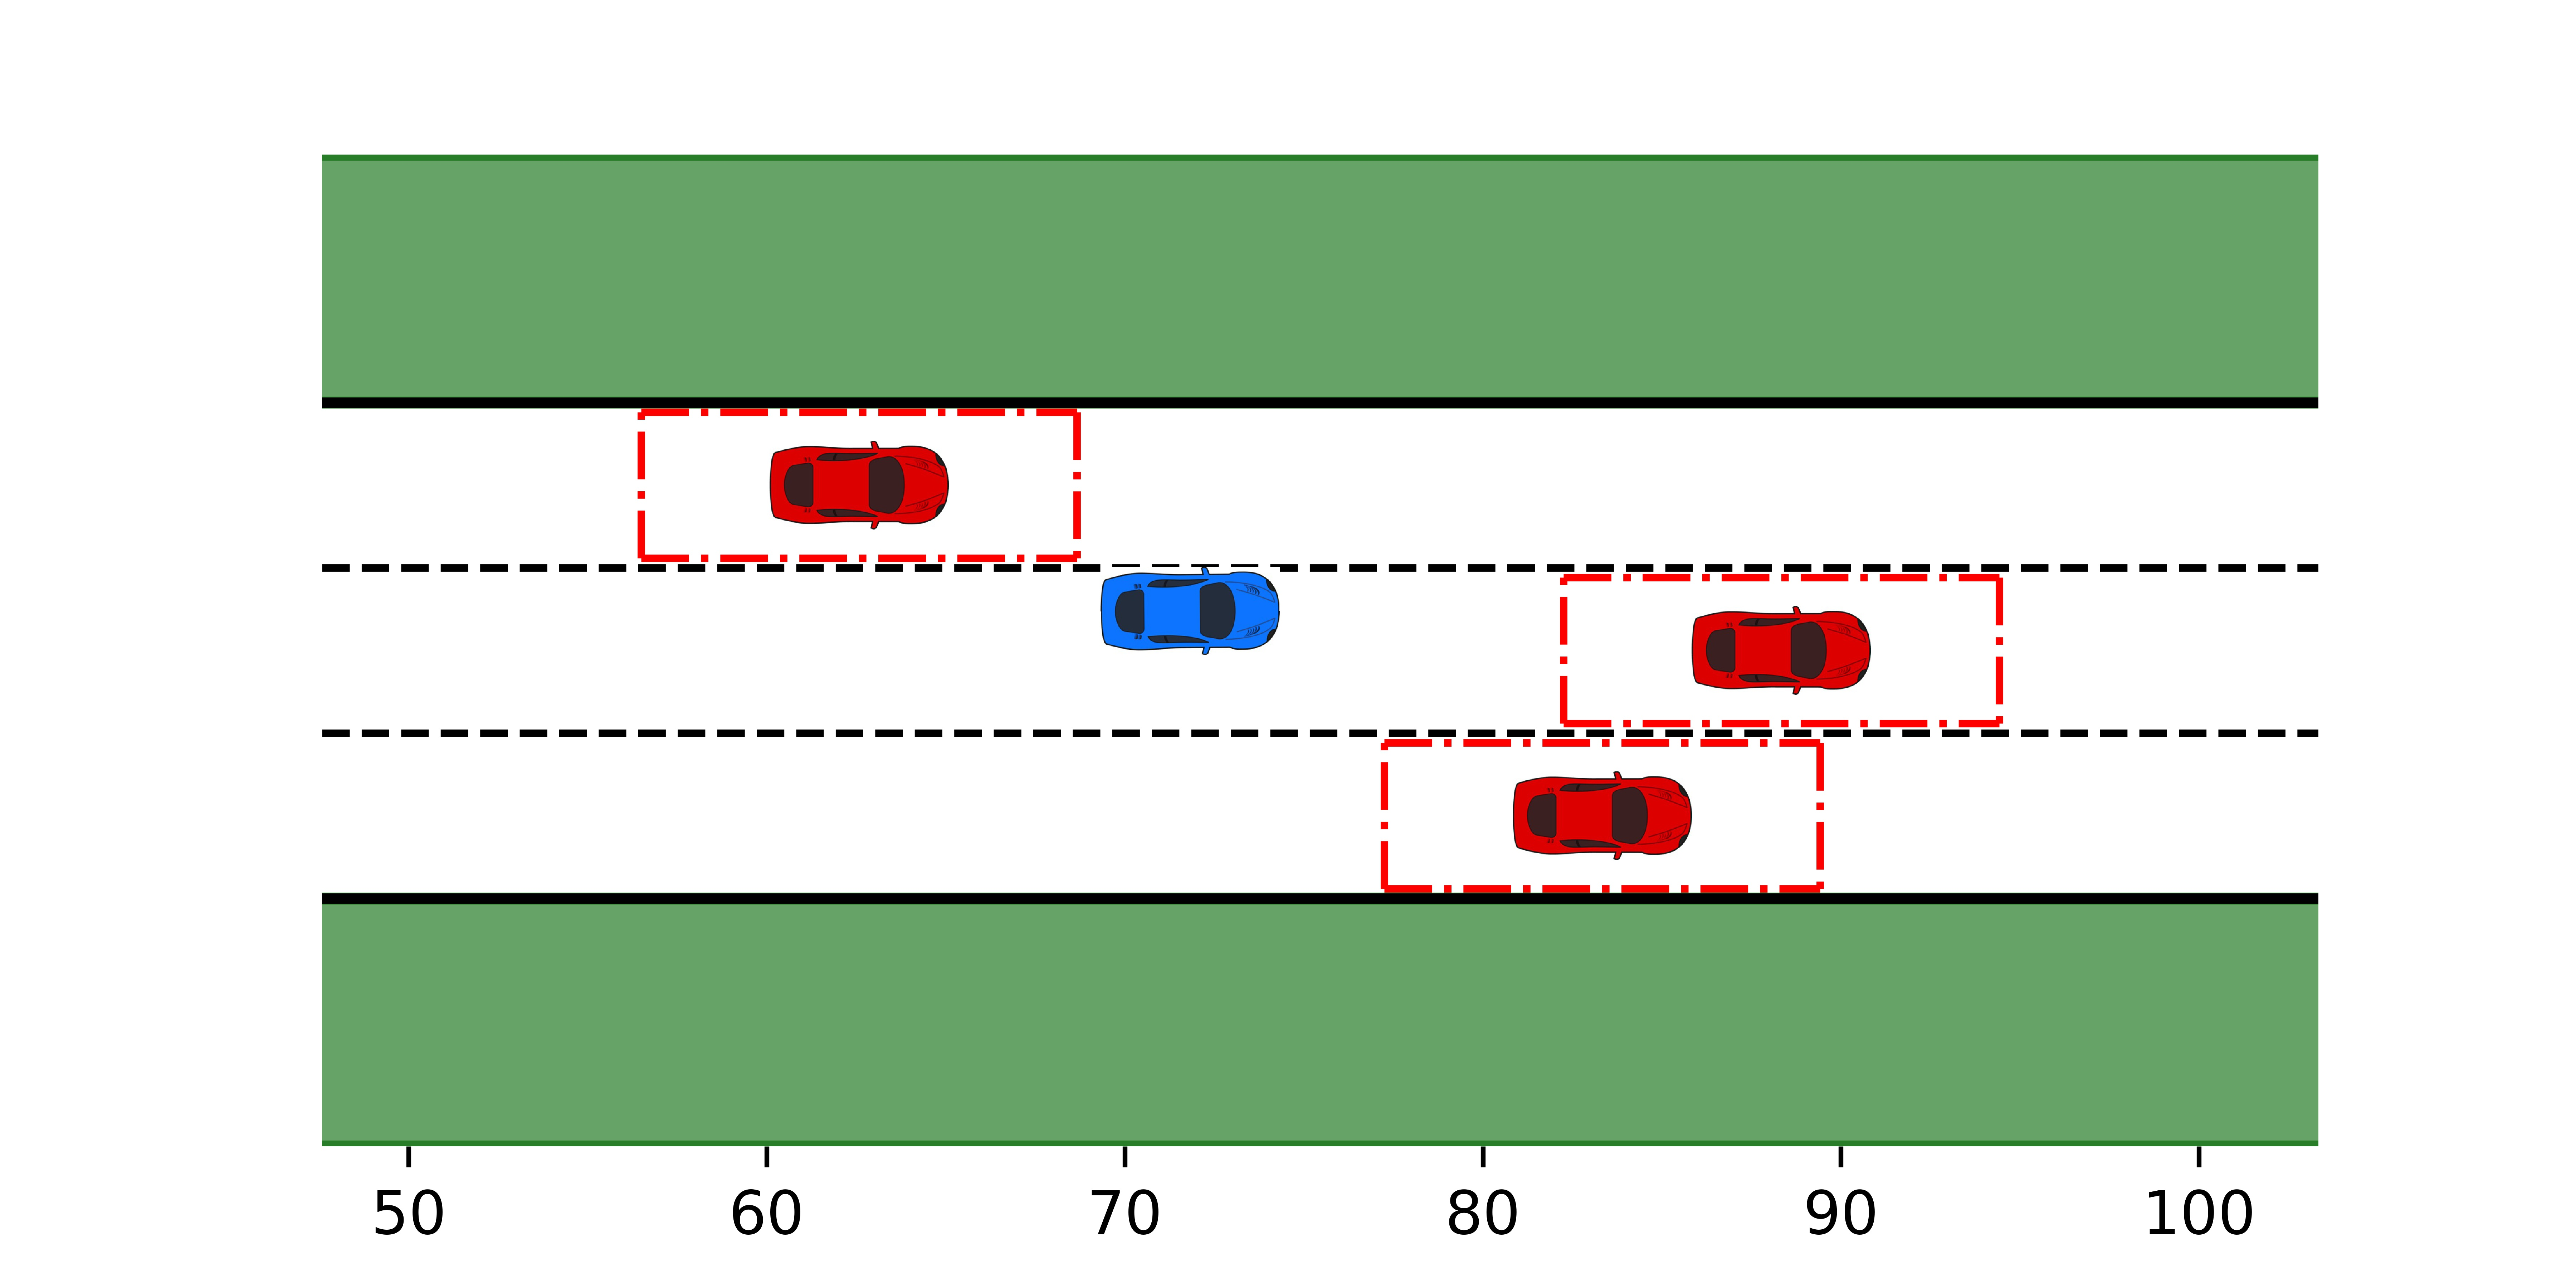
\includegraphics[clip, trim = {1.5cm 0.25cm 1.5cm 0.25cm}]{plot_con6.jpg}};
			
			\node (adp5)[below  = 1.cm of adp4, minimum width = 0.cm, minimum height = 0cm, inner sep = 0pt]{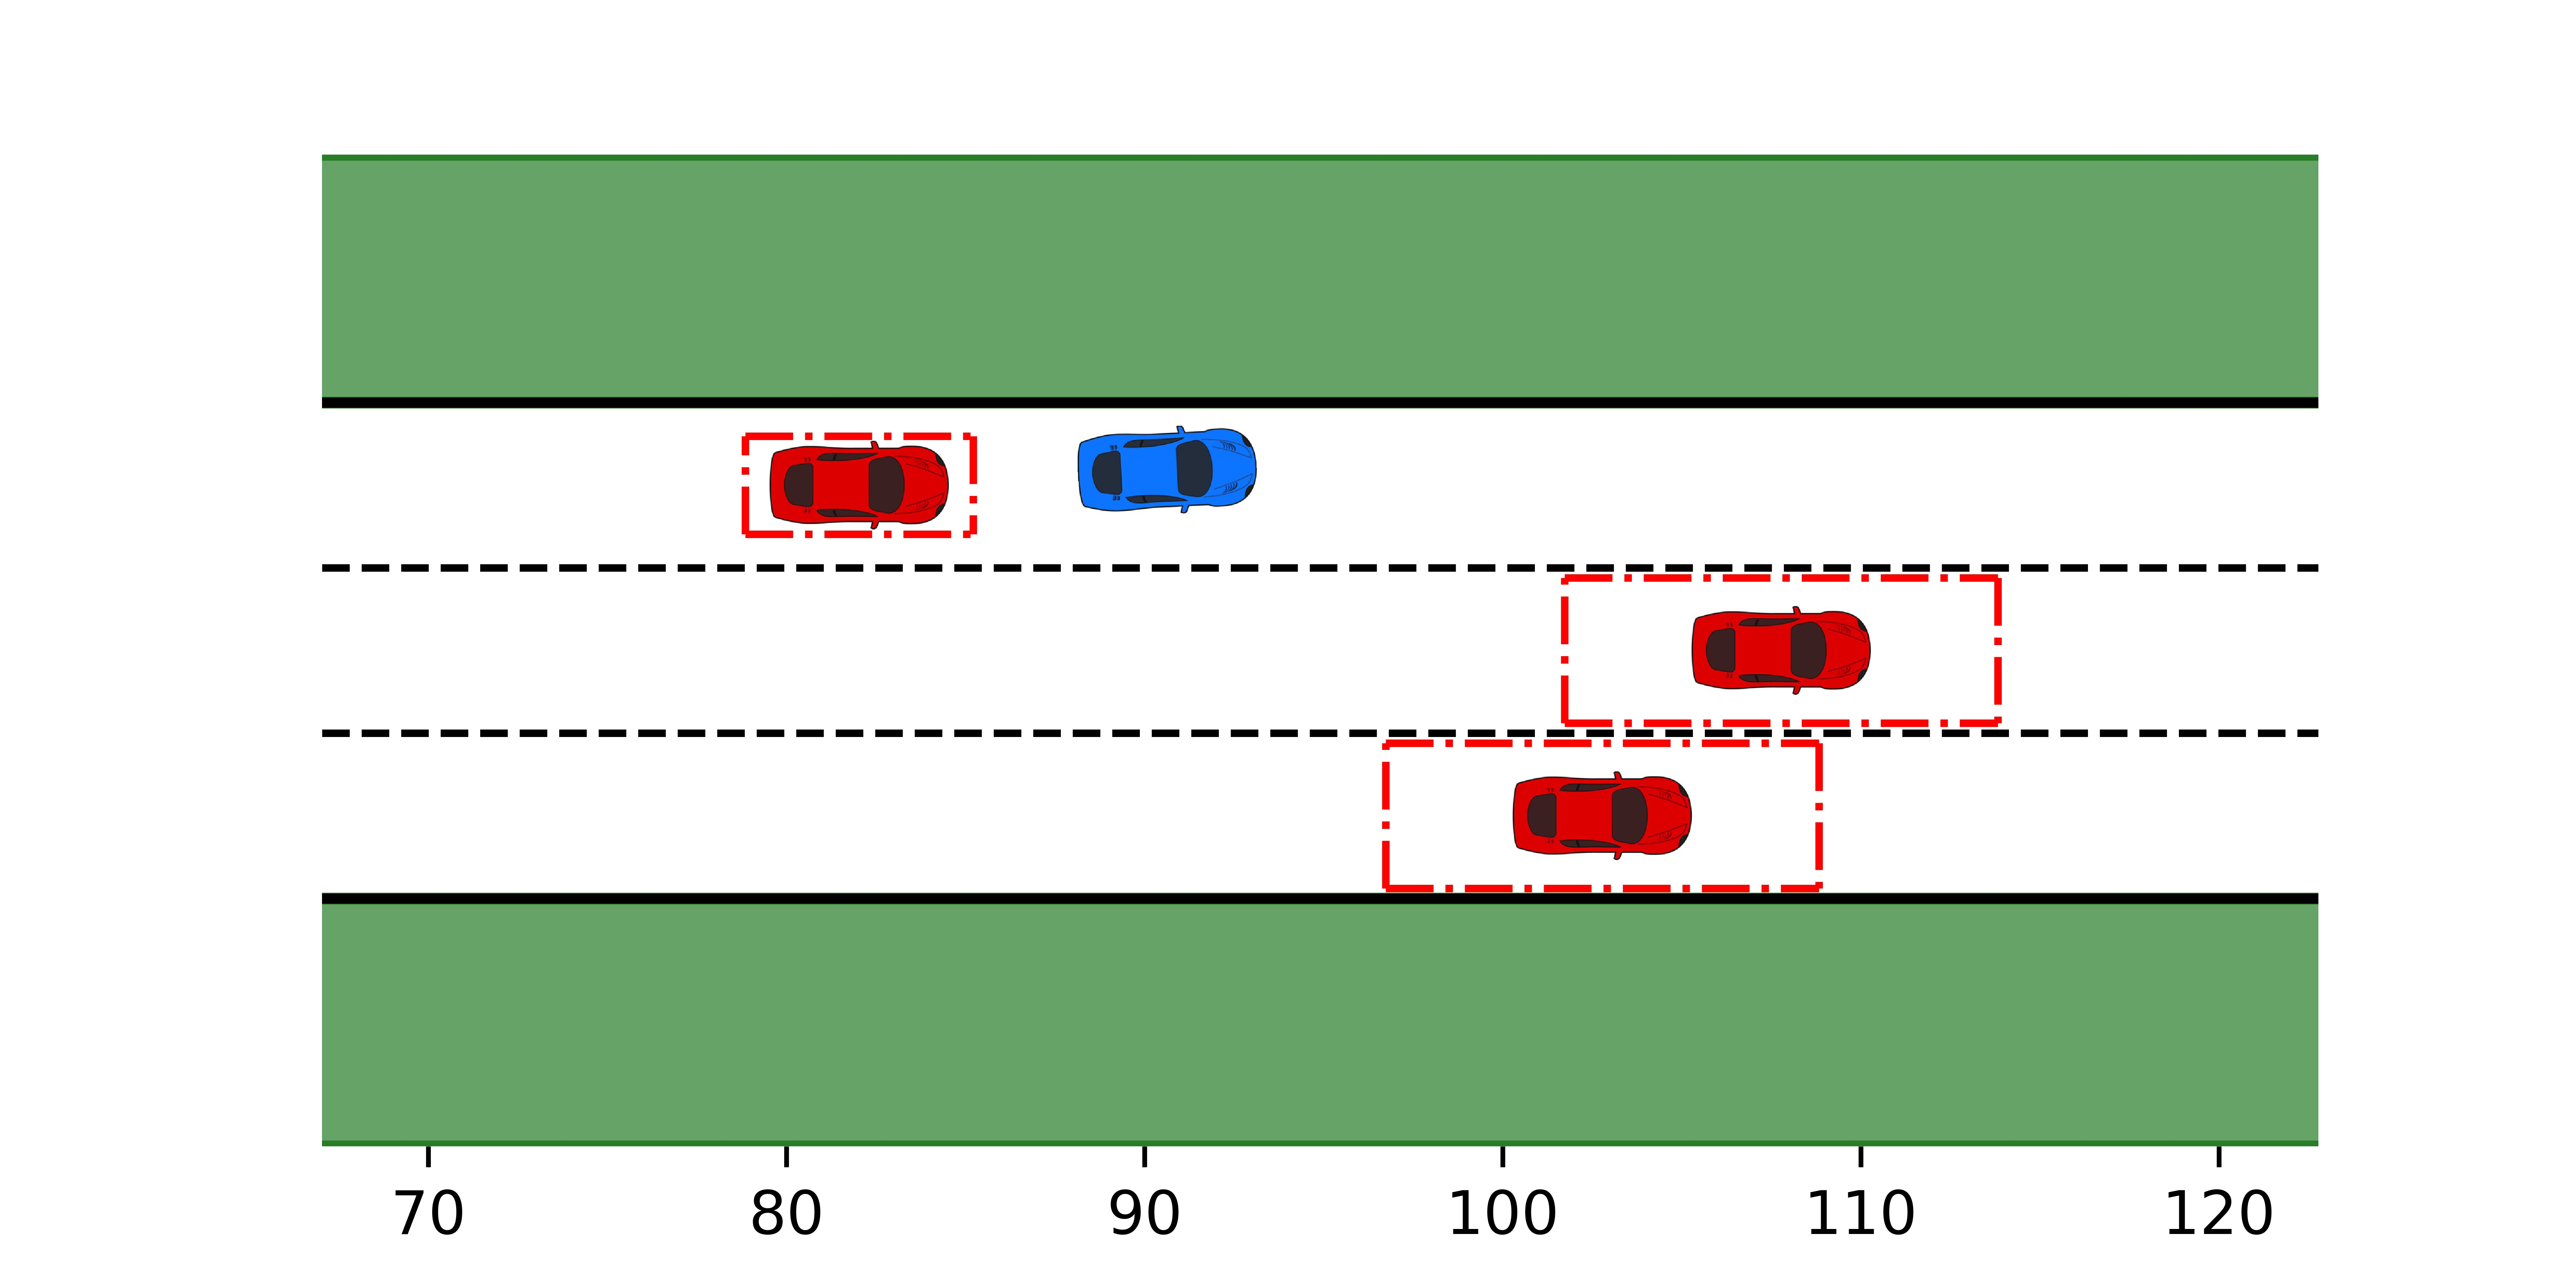
\includegraphics[clip, trim = {1.5cm 0.25cm 1.5cm 0.25cm}]{plot_adp8.jpg}};
			\node (agg5)[left = 1cm of adp5, minimum width = 0.cm, minimum height = 0cm, inner sep = 0pt]{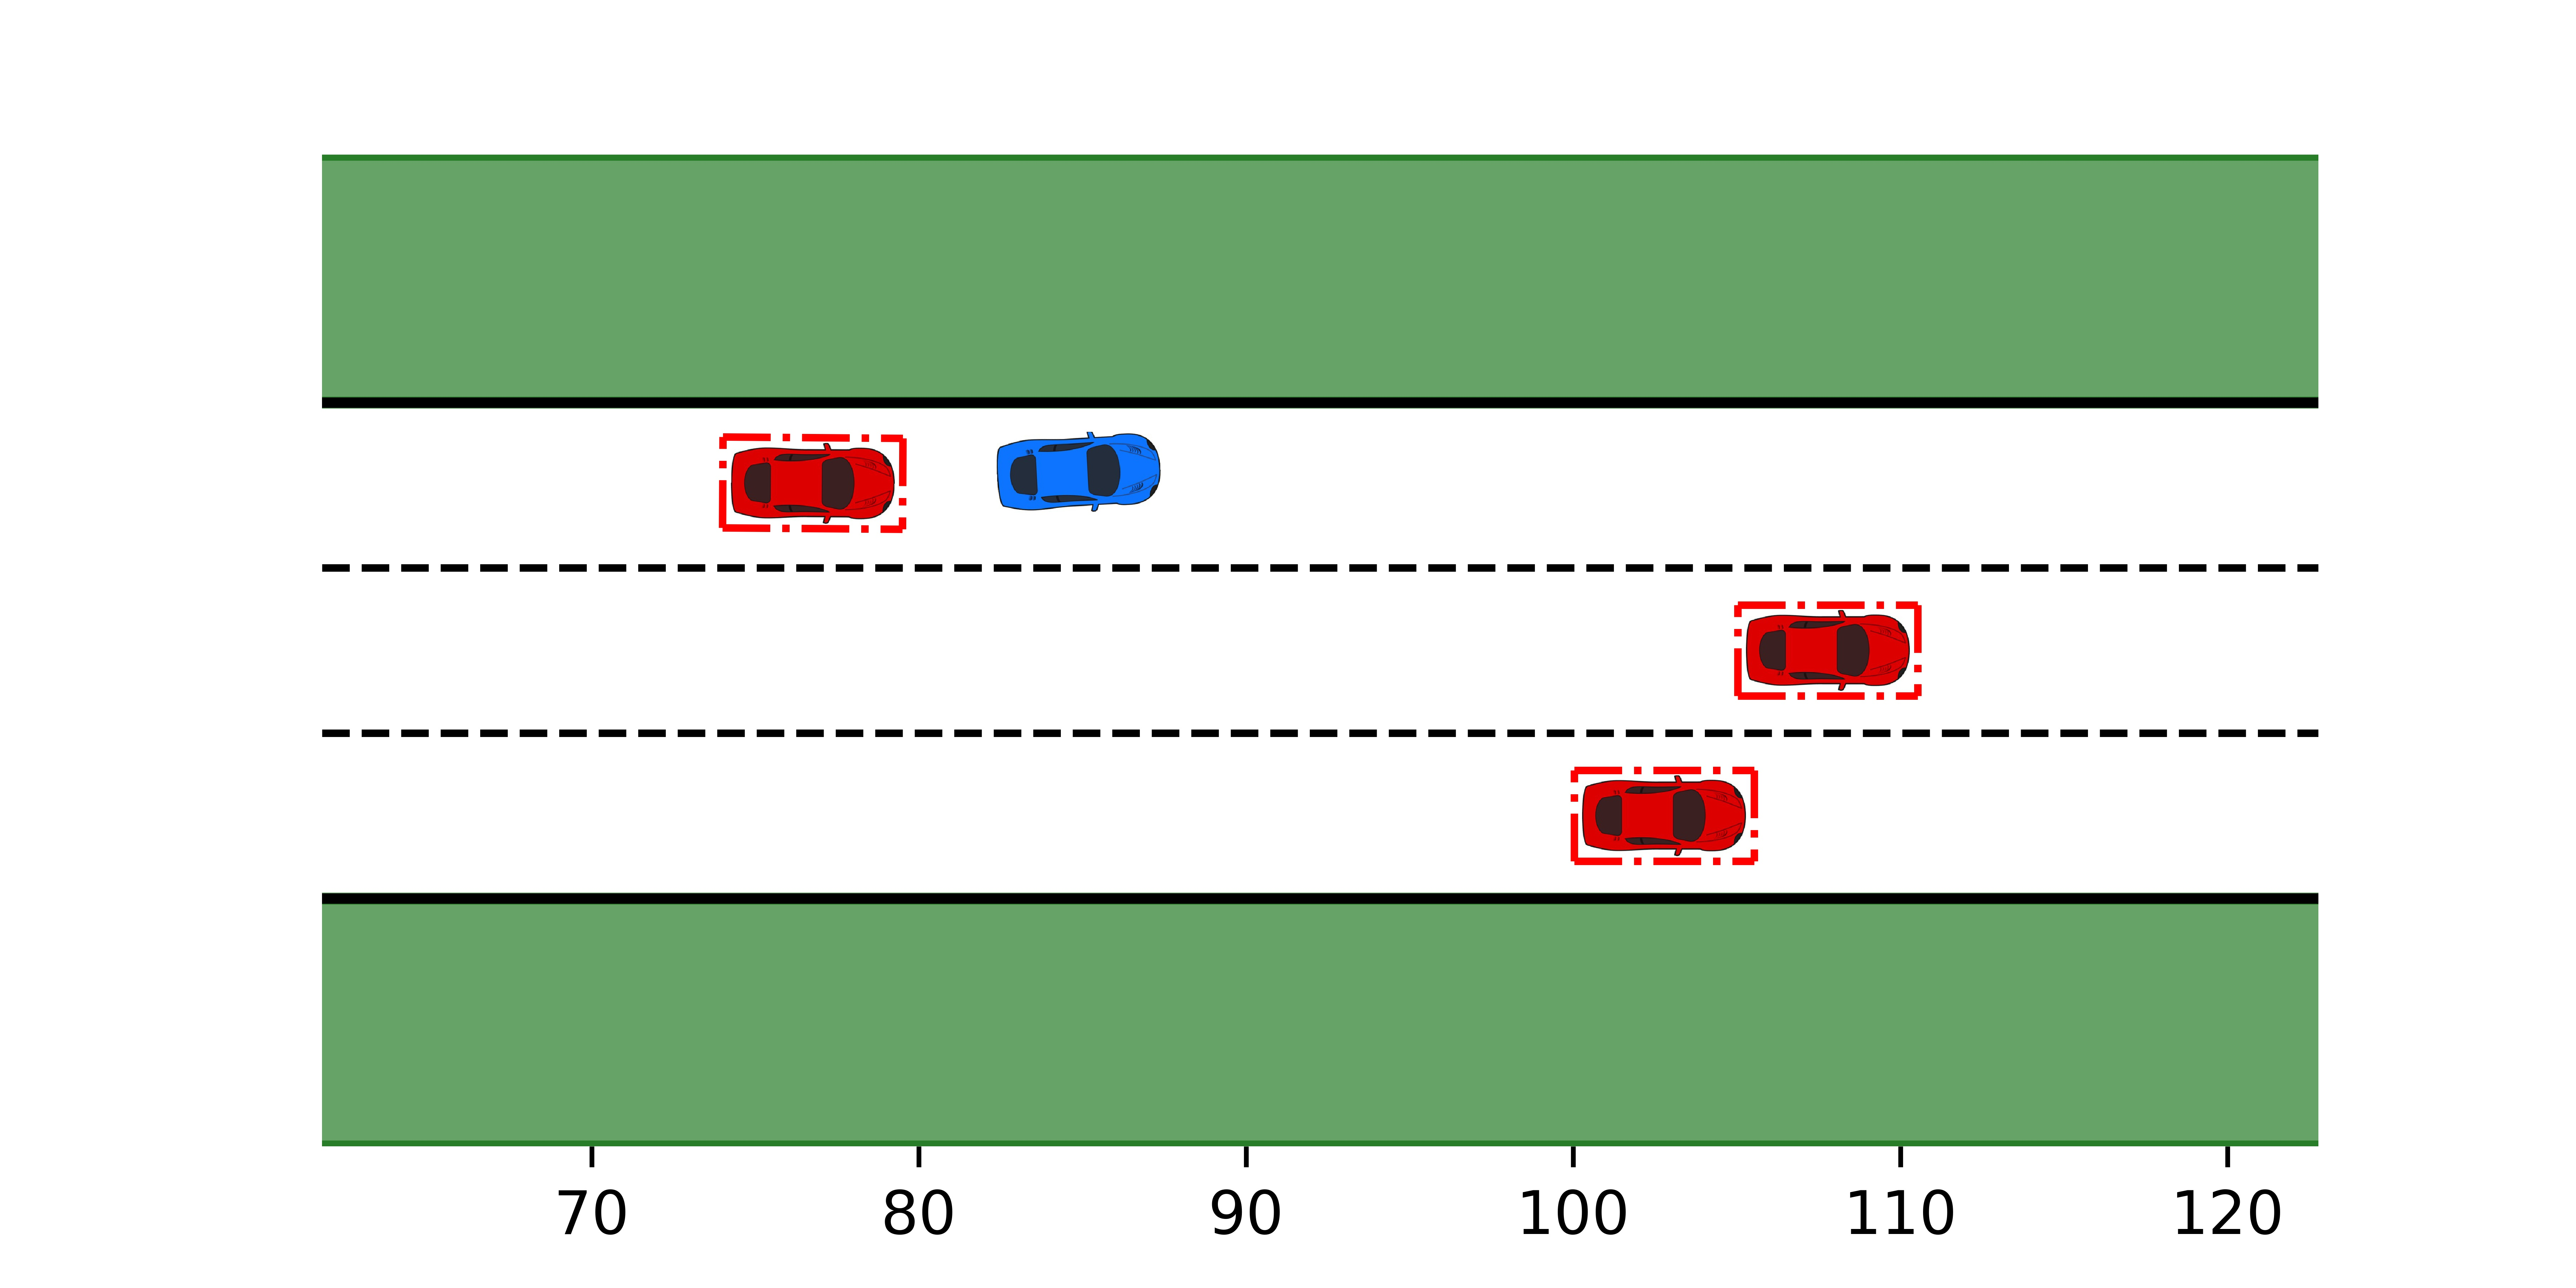
\includegraphics[clip, trim = {1.5cm 0.25cm 1.5cm 0.25cm}]{plot_agg8.jpg}};
			\node (con5)[ right = 1cm of adp5, minimum width = 0.cm, minimum height = 0cm, inner sep = 0pt]{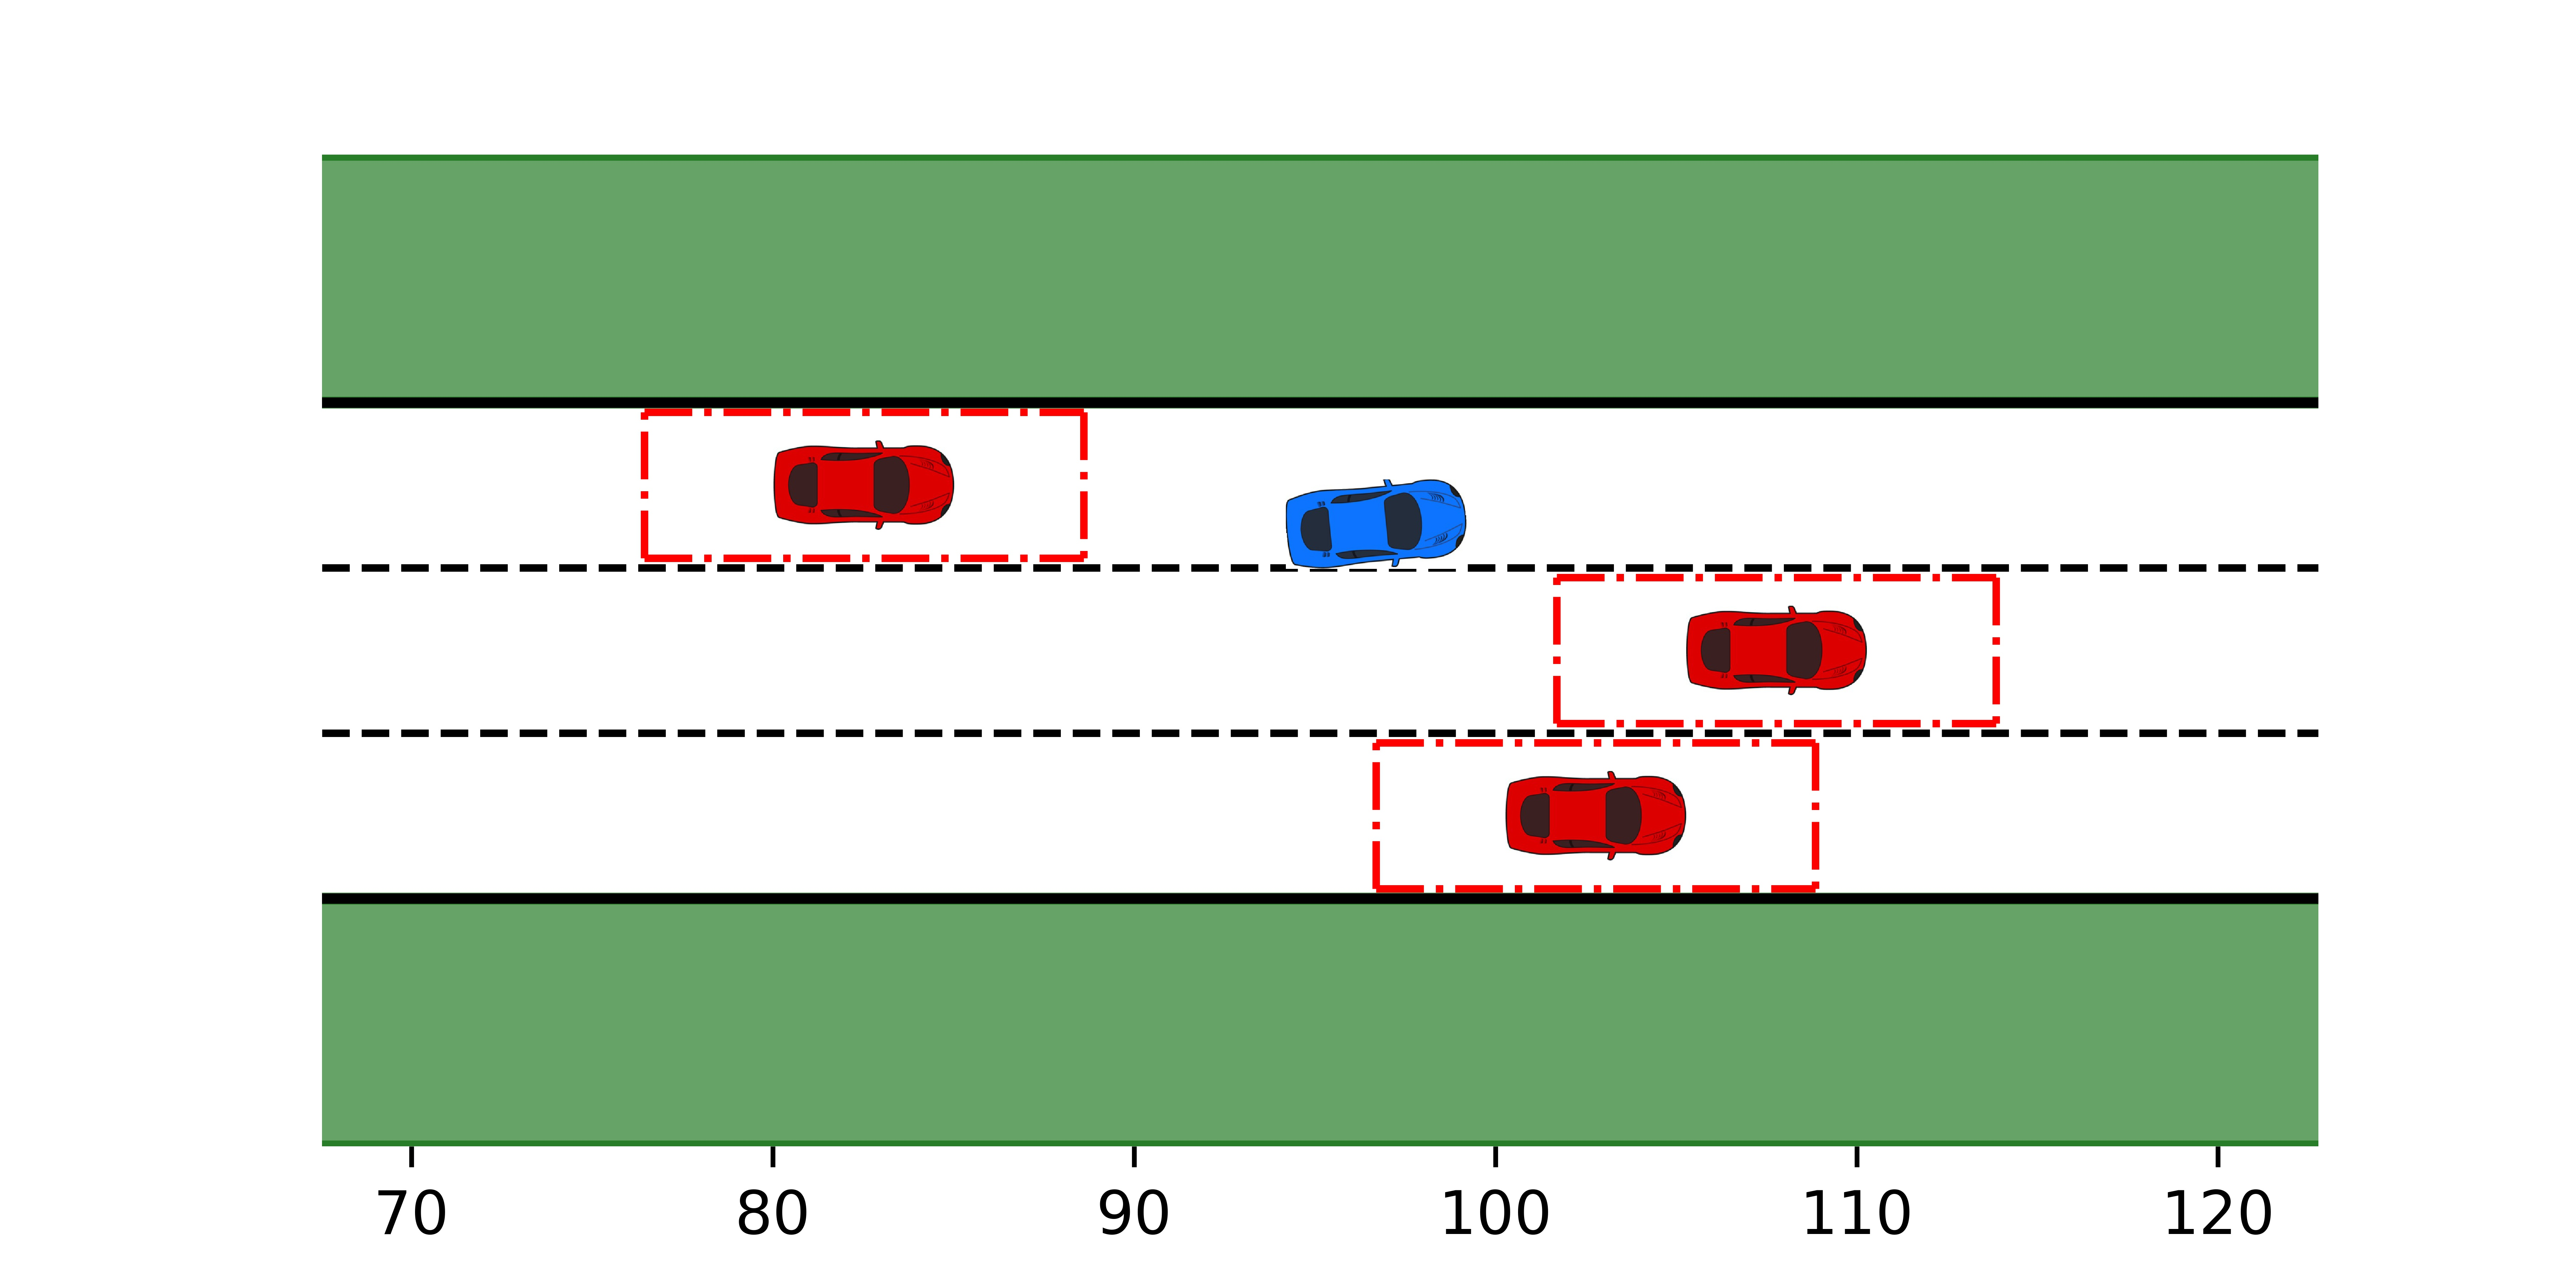
\includegraphics[clip, trim = {1.5cm 0.25cm 1.5cm 0.25cm}]{plot_con8.jpg}};
			%			
			%			\node (adp6)[below  = 1.5cm of adp5, minimum width = 0.cm, minimum height = 0cm, inner sep = 0pt]{\includegraphics[clip, trim = {1.5cm 0.25cm 1.5cm 0.25cm}]{plot_adp10.jpg}};
			%			\node (agg6)[left = 1cm of adp6, minimum width = 0.cm, minimum height = 0cm, inner sep = 0pt]{\includegraphics[clip, trim = {1.5cm 0.25cm 1.5cm 0.25cm}]{plot_agg10.jpg}};
			%			\node (con6)[ right = 1cm of adp6, minimum width = 0.cm, minimum height = 0cm, inner sep = 0pt]{\includegraphics[clip, trim = {1.5cm 0.25cm 1.5cm 0.25cm}]{plot_con10.jpg}};
			
			
			\node (xlabeladp) [below = 1cm of adp5, inner sep = 0pt] {\Huge Distance (m)};
			\node (xlabelagg) [below = 1cm of agg5, inner sep = 0pt] {\Huge Distance (m)};
			\node (xlabelcon) [below = 1cm of con5, inner sep = 0pt] {\Huge Distance (m)};
			
			
			\node (t0) [left = 0.25cm of agg1, inner sep = 0pt] {\Huge $t=0 s$};
			\node (t1) [left = 0.25cm of agg2, inner sep = 0pt] {\Huge $t=1 s$};
			\node (t2) [left = 0.25cm of agg3, inner sep = 0pt] {\Huge $t=2 s$};
			\node (t3) [left = 0.25cm of agg4, inner sep = 0pt] {\Huge $t=3 s$};
			\node (t4) [left = 0.25cm of agg5, inner sep = 0pt] {\Huge $t=4 s$};
			
			\node (agg) [above = 0.25cm of agg1, inner sep = 0pt] {\Huge (a) Aggressive};
			\node (adp) [above = 0.25cm of adp1, inner sep = 0pt] {\Huge (b) Adaptive};
			\node (con) [above = 0.25cm of con1, inner sep = 0pt] {\Huge (c) Conservative};
			
			
			\end{tikzpicture}
			\par\end{centering}
		\protect\caption{.}
		\label{fig:snapshots}
	\end{figure*}

	\begin{figure}
		\begin{centering}
			\begin{tikzpicture}[scale=0.5,transform shape]
			\node (origin) at (0,0) {};
			
			\node (fig)[below left = 0cm and 0cm of origin, minimum width = 0.cm, minimum height = 0cm, inner sep = 0pt]{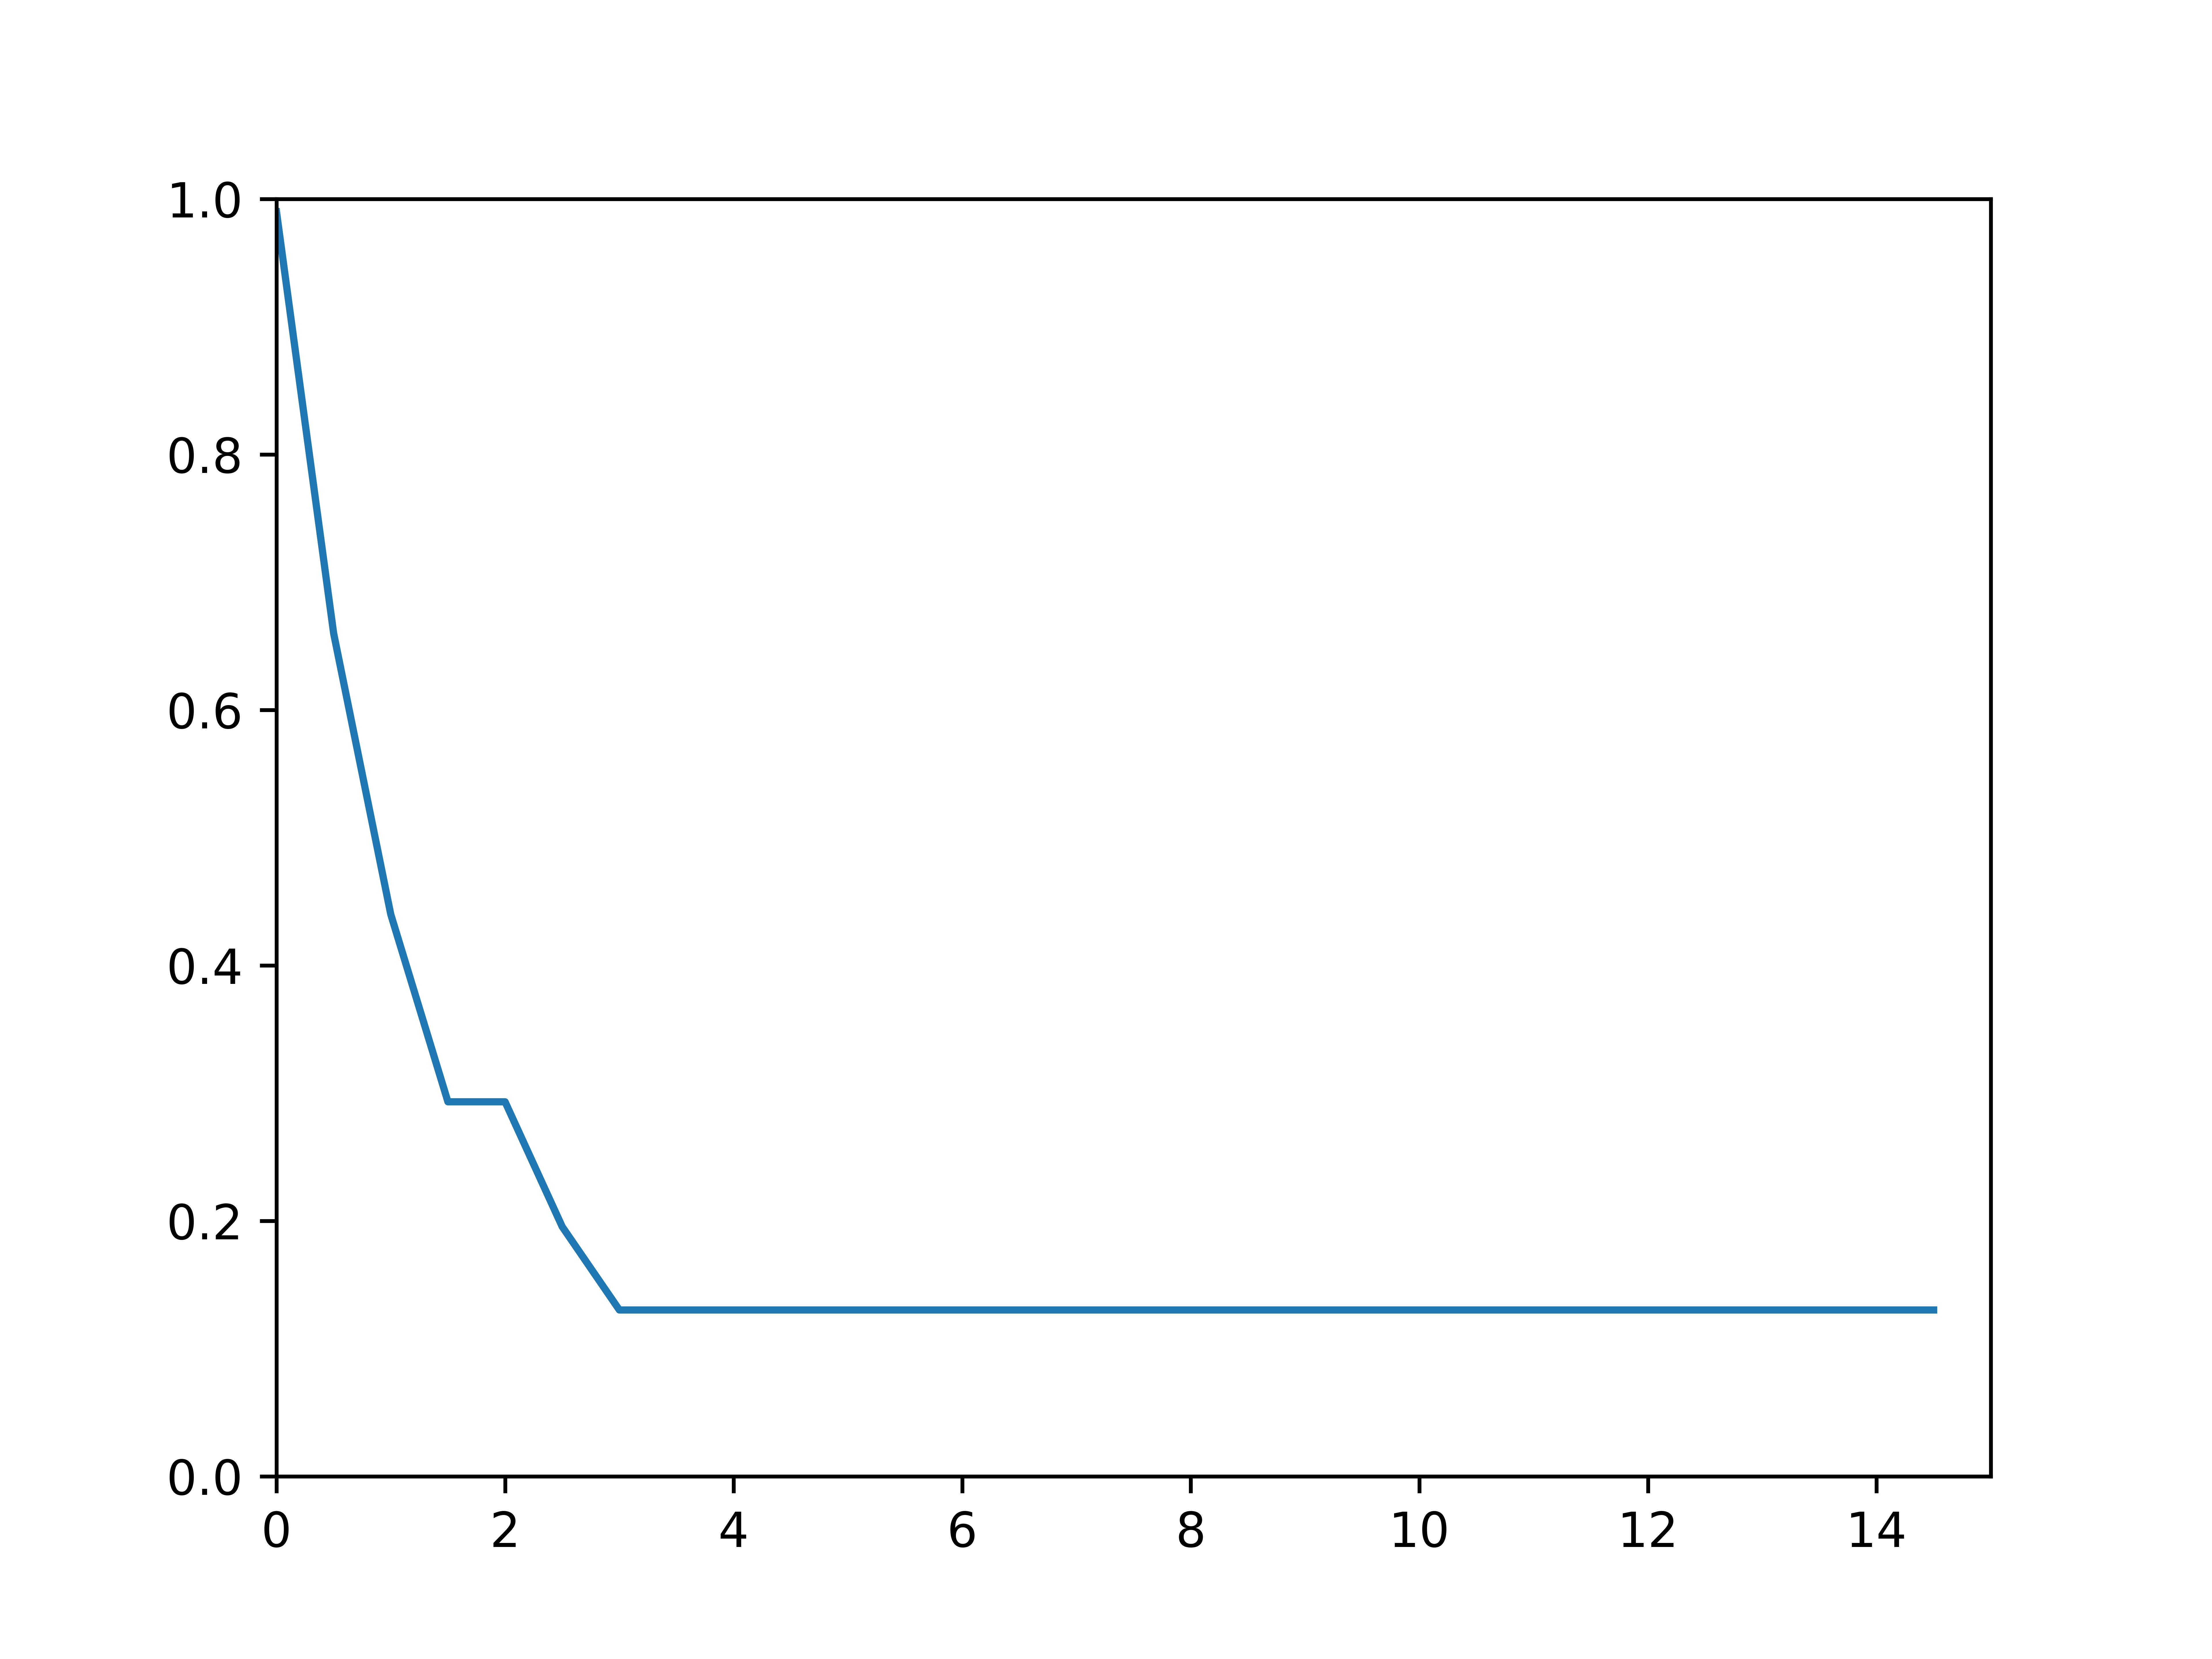
\includegraphics[clip, trim = {1.25cm 0.8cm 1.5cm 1.25cm}]{level_ratio_history_adp29.jpg}};
			
			\node (xlabel) [below = 0.5cm of fig, inner sep = 0pt] {\LARGE Time (s)};
		
			\node (ylabel) [below left = -6.1cm and 1cm of fig, inner sep = 0pt, rotate = 90] {\huge $P_{K_{4}^2 = 0}$};
			
			\end{tikzpicture}
			\par\end{centering}
		\protect\caption{Probability that vehicle 4 can be modeled as level-0 from the perspective of the ego vehicle.}
		\label{fig:level_history}
	\end{figure}
	
	
	
	%==========================================================================%
	
	\section{Conclusions}
	\label{sec:conclusions}
	We proposed the robust decision-making strategy for autonomous vehicles when they share the road with the other road participants.We modeled the vehicle interactions using a level-k framework, then the decision of the autonomous vehicle was made based on the identified other vehicle's level in real-time. To avoid the conservative or aggressive behavior of autonomous vehicle, the accuracy of the level estimation was utilized to represent the uncertainty bounds of the interactive vehicles. Based on updated level estimation accuracy, the uncertainty bounds could be adjusted, and autonomous vehicle adaptively plans its motion for a given prediction horizon. Through the simulation verification, we could observe the reasonable behavior of autonomous vehicle, compared to the behaviors of conventional decision-making approaches. However, extending to handle the large number of vehicles has not been researched in this study, and computational challenge is anticipated. For the future research, we address computational tractability when the more number of interactive vehicles is given.

	%==========================================================================%

	\section*{Acknowledgement}
	We would like to express out appreciation to Anouck Girard and Nan Li who provided expertise that greatly assisted the research and it should be noted that the code publicly available (\url{https://github.com/gokulsivasankar/RobustDecisionMaking}) is based on his previous study \cite{Li2018}.



	%==========================================================================%

	\bibliographystyle{ieeetr}
	\bibliography{Reference}
	
	%	\noindent where  $t$ denotes the discrete time instant; the pair $\left(x\left(t\right),\,y\left(t\right)\right)$ $\left[\SI{}{\meter}\right]$ represent the global position of the center of mass of the vehicle; the vehicle's speed is denoted by $v\left(t\right)$ $\left[\SI{}{\meter \per \second}\right]$; 	$\beta\left(t\right)$ $\left[\SI{}{\radian}\right]$ is the angle of $v\left(t\right)$ with respect to the longitudinal axis of the vehicle; $\psi\left(t\right)$ $\left[\SI{}{\radian}\right]$ denotes the vehicle’s yaw angle (the angle between the vehicle’s heading direction and the global x-direction); $a\left(t\right)$ $\left[\SI{}{\meter \per \second^2}\right]$ denotes the vehicle’s acceleration at time $t$;  $\Delta t$ $\left[\SI{}{\second}\right]$ denotes the time step size; $\delta_f\left(t\right)$ $\left[\SI{}{\radian}\right]$ represents the front steering angle; and  $l_f$ $\left[\SI{}{\meter}\right]$ and $l_r$  $\left[\SI{}{\meter}\right]$ are the distance of the center of the mass of the vehicle to the front and rear axles, respectively; $w_x\left(k\right)$ $\left[\SI{}{\meter}\right]$  and $w_x\left(k\right)$ $\left[\SI{}{\meter}\right]$ denote the uncertainty in the position of the center of mass, respectively. It is assumed the uncertainties originate from a closed and compact disturbance set, ${\mathcal{W}} \coloneqq  \left\{ w = \left(w_x,\,w_y\right) |\zeta w\leq\theta,\,\zeta\in\mathbb{R}^{a\times 2},\,\theta\in\mathbb{R}^{b}\right\}$, with $b \in 2\mathbb{Z}^{+}$. The disturbance set is assumed to contain the origin. Furthermore, it is assumed that the rear wheels cannot be steered. The acceleration, $a\left(t\right)$, and the front steering angle, $\delta_f\left(t\right)$, are the two inputs. At a given time instant, the vehicle selects the inputs from an action set as described below.
	
\end{document}